% PEV description

\chapter{Persuasive Electric Vehicle (PEV)}
\label{ch:pev}

PEV has already been presented in (\autoref{ch:intro}), as a lightweight, low--cost, electric and autonomous platform, that would operate in the intersection of AVs (\autoref{fig:pevstreet}) and bicycle sharing services.
\begin{figure}[h]
  \centering
  \frame{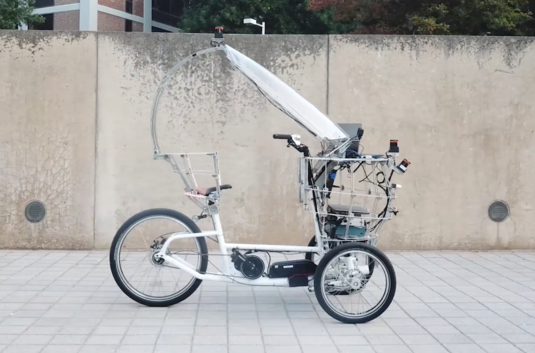
\includegraphics[width=.95\linewidth]{pictures/05/pev_street}}
  \caption{PEV from the side}
  \label{fig:pevstreet}
\end{figure}

In this chapter, a more technical report of the vehicle will be done, as well as results from the SLAM on the different environments selected for the PEV.

\section{Description of the vehicle}


\subsection{General specifications}
The PEV weights 50 kg in vacuum is composed of of 2 main parts:
\begin{itemize}
  \item \textbf{Steel base:} The white rickshaw shown in \autoref{fig:pevstreet} is made of stainless steel and weights 30 kg (including wheels). It connects to all three wheels and housess  both motors and the battery.

  \item \textbf{Aluminum frame}: The exterior part of the PEV is made in aluminum sheets that weight in total 10 kg. The front part forms a curved shape and inside it houses the sensor batteries, power supply and connections.
\end{itemize}

The maximum load it could carry is around 120 kg which is enough to carry most people or a notable amount of packages, therefore it could accomplish its 2 main goals: people mover and package delivery.

The PEV would eventually operate on bike lanes, therefore speed is limited to 20 km/h, but the maximum speed the engine can achieve is up to 30 km/h.

The engine is fed with 10 Ah Lithium-Ion battery that can provide an autonomoy of 40 km. Sensors powered through a different system and can last for 1 hour without recharging.

Last, the PEV is provided with cellular communication so that it can communicate with remote machines and receive updates on the system.

The general details of the PEV are summarized on \autoref{tab:pevdescr}
\begin{table}[h!]
  \centering
  \begin{tabular}{ll}
    \hline
    \textbf{Parameter}             & \textbf{Value}  \\ \hline
    \textbf{Weight (kg)}           & 50.0            \\ \hline
    \textbf{Max. load (kg)}        & 120.0           \\ \hline
    \textbf{Max. speed (km/h)}     & 30              \\ \hline
    \textbf{Avg. speed (km/h)}     & 20.0            \\ \hline
    \textbf{Battery Capacity (Ah)} & 10.0            \\ \hline
    \textbf{Autonomy (km)}         & 40              \\ \hline
    \textbf{Autonomy (h)}          & 1               \\ \hline
    \textbf{Communications}        & 4G LTE cellular \\ \hline
  \end{tabular}
  \caption{Specifications for the PEV}
  \label{tab:pevdescr}
\end{table}

\subsection{Hardware and sensors}

In the following paragraphs, all the components that conform the system will be described:
\parunder{Sensors} The PEV has the following sensors:
\begin{itemize}
  \item \textbf{Lidar} PEV has 3 lidars installed: 1 3D lidar and 2 2D lidars (\autoref{fig:pevlidars}).
  \begin{itemize}
    \item \href{https://velodynelidar.com/vlp-16.html}{Velodyne VLP16}: This 3D lidar has a 100 m range, with a 360\textdegree field of view and generally rotates at 600 rpm. it has 16 channels covering an angle of $\pm 15$\textdegree and generates 600.000 points per second. Tha main use of this lidar is to perform both SLAM and localization.

    \item \href{https://www.hokuyo-aut.jp/search/single.php?serial=169}{Hokuyo UTM-30LX}: There are 2 lidars of this kind one located at 0\textdegree and the other tilted 30\textdegree. They are mainly employed for obstacle detection but they can be used as input for 2D SLAM algorithms. The field of view is of 270\textdegree producing  57.600 points per second.
  \end{itemize}
  \begin{figure}[ht]
    \centering
    \subfloat[Velodyne VLP16]{\frame{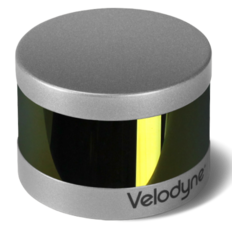
\includegraphics[width=.40\linewidth]{pictures/05/puck}}} \qquad
    \subfloat[Hokuyo UTM-30LX]{\frame{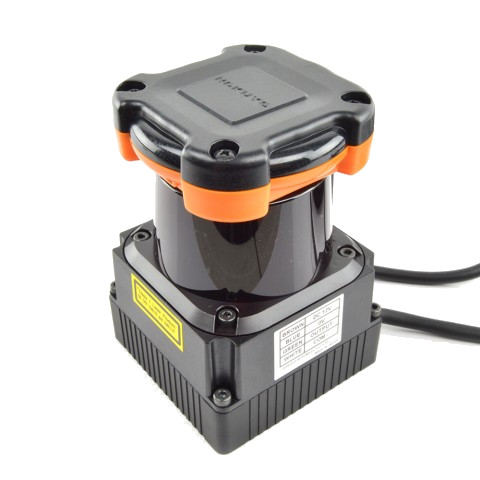
\includegraphics[width=.40\linewidth]{pictures/05/hokuyo30}}}
    \caption{Lidars installed on the PEV}
    \label{fig:pevlidars}
  \end{figure}

  \item \textbf{Cameras} The PEV has 2 different types of cameras:
  \begin{itemize}
    \item \underline{Monocular cameras}: 4 \href{https://www.logitech.com/en-us/product/hd-pro-webcam-c920}{Logitech C920} are located on top of the aluminum frame in such a way to have a 360\textdegree field of view. These cameras are used to perform object recognition and traffic light detection.

    \item \underline{Stereo cameras}: 2 \href{https://www.stereolabs.com/}{ZED cameras} are mounted on the PEV, one of the front and one on the back. They are used for short range recognition, lane detection and they provide odometry estimates.
  \end{itemize} 

  \item \textbf{Encoders}: The PEV has 2 encoders located on the back wheel and the steering bar. Their signals are then translated to speed commands according to the Ackermann steering equations.

  \item \textbf{Inertial Measurement Units}: Two \href{https://www.xsens.com/products/mti-1-series/}{Xsens MTi-1} IMUs (\autoref{fig:pevsens}\protect\subref{fig:imu}) are located on the front of the PEV, one horizontal to the floor plane and one tilted 30\textdegree downwards. These devices measure acceleration, orientation and magnetic field, and are fused with the encoders and GPS to improve the accuracy of state estimation.   

  \item \textbf{GPS}: PEV has a \href{https://docs.emlid.com/reach/}{Emlid Reach RTK GPS} receiver with Real Time Kinematics (RTK) functionality and that achieves precisions of centimeters (\autoref{fig:pevsens}\protect\subref{fig:gps}).

  \begin{figure}[h]
    \centering
    \subfloat[IMU]{\frame{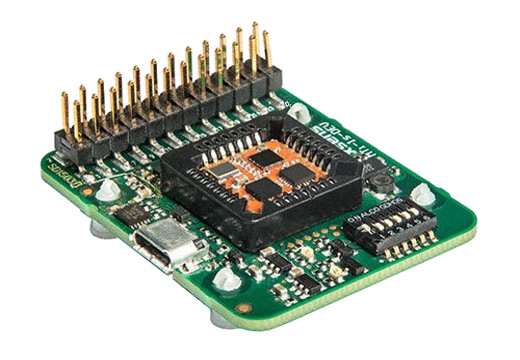
\includegraphics[width=.40\linewidth]{pictures/05/xsens}}\label{fig:imu}} \qquad
    \subfloat[GPS receiver]{\frame{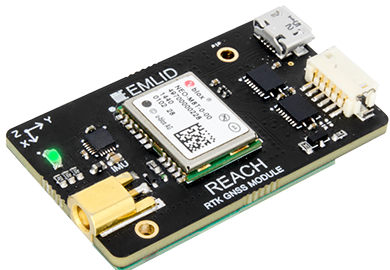
\includegraphics[width=.40\linewidth]{pictures/05/emlid}}\label{fig:gps}}
    \caption{Two types of sensors installed on the PEV}
    \label{fig:pevsens}
  \end{figure}
\end{itemize}

\parunder{Actuators} The main actuators of the PEV have alreayd been defined: The \textbf{middrive} engine and the \textbf{steering} motor. Both are controlled by a \textbf{'Vedder' Electric Speed Control (VESC)} which is an open--source speed control just as shown in \autoref{fig:vesc}. Apart from controlling motors, it allows to control servos and read from pulse encoders.
\begin{figure}[h]
  \centering
  \frame{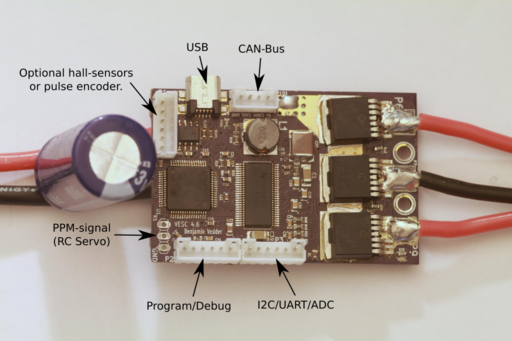
\includegraphics[width=\linewidth]{pictures/05/vesc}}
  \caption{\href{https://vesc-project.com/}{VESC} electronic circuit}
  \label{fig:vesc}
\end{figure}

The parameters for both motors can be configured using the \href{http://vedder.se/2015/01/vesc-open-source-esc/}{BLDC tool} provided by the same company and shown in \autoref{fig:bldc}. This software module also provides visualization tabs to check the state of the system.
\begin{figure}[h]
  \centering
  \frame{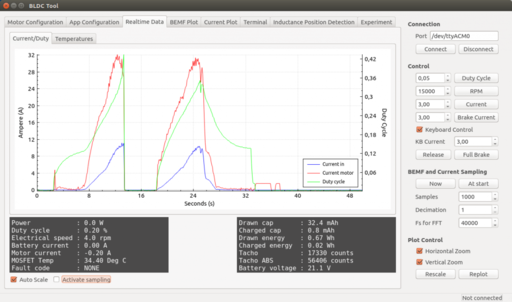
\includegraphics[width=\linewidth]{pictures/05/bldc}}
  \caption{BLDC tool to configure VESC}
  \label{fig:bldc}
\end{figure}

In order to \textbf{brake}, the PEV also features a \textbf{servo motor} attached to the rear wheel that pulls the break when actuated. It is also controlled by the middrive VESC module.

\parunder{Power supply} As for the power system of the PEV, there are 2 main sources:
\begin{itemize}
  \item \textbf{Lithium--Ion battery}: This battery powers the middrive engine, operates at 48 V and has 10 Ah of charge.

  \item \textbf{Lead--Acid batteries}: There are 4 12 V lead--acid batteries mounted on the PEV. 2 of them are mounted in series and are attached to the steering motor. The other 2 are connected in parallel and run the sensors, USB hubs and computers.
\end{itemize}

\parunder{Computing} The 'brains' of the PEV are divided into:
\begin{itemize}
  \item \textbf{Jetson TX2}: There is one Jetson TX2 that takes the input of the four cameras and publishes it on the system. To process large images at high speed, this Jetson TX2 is connected to a PCI express module with four USB 3.0 ports just as shown on \autoref{fig:pcie}
  \begin{figure}[h]
    \centering
    \frame{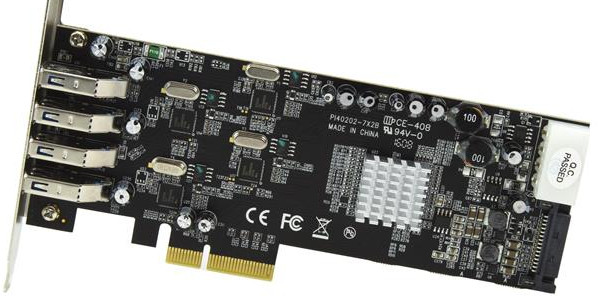
\includegraphics[width=.7\linewidth]{pictures/05/pcie}}
    \caption{PCI express module}
    \label{fig:pcie}
  \end{figure}

  \item \textbf{Laptop}: The main computer is a Dell Precision 5520 with an 3.0 GHz \href{https://ark.intel.com/products/97463/Intel-Xeon-Processor-E3-1505M-v6-8M-Cache-3_00-GHz}{Intel Xeon E3-1505M CPU}, 16 GB DDR4 RAM and \href{https://www.nvidia.com/content/dam/en-zz/Solutions/design-visualization/documents/quadro-mobile-pro-graphics-line-card-us-r1-hr.pdf}{Nvidia Quadro M1200 4 GB} Graphics Processing Unit (GPU).
\end{itemize}

\parunder{Communication} PEV has wireless communications thanks to an \href{https://www.tp-link.com/la/products/details/cat-4691_TL-MR6400.html}{TP--Link TL-MR6400} router to which a generic SIM card can be attached, adding 4G LTE connectivity to the PEV.

\section{Setup}

A conceptual overview of the PEV's setup is shown in \autoref{fig:pevsetup}. It is more complex than the Nexus robot but it shares the same principles. Sensors are handled by the laptop except for the cameras, and the computing units send commands to the actuators. 
\begin{figure}[t!]
  \centering
  \makebox[\linewidth]{
    \frame{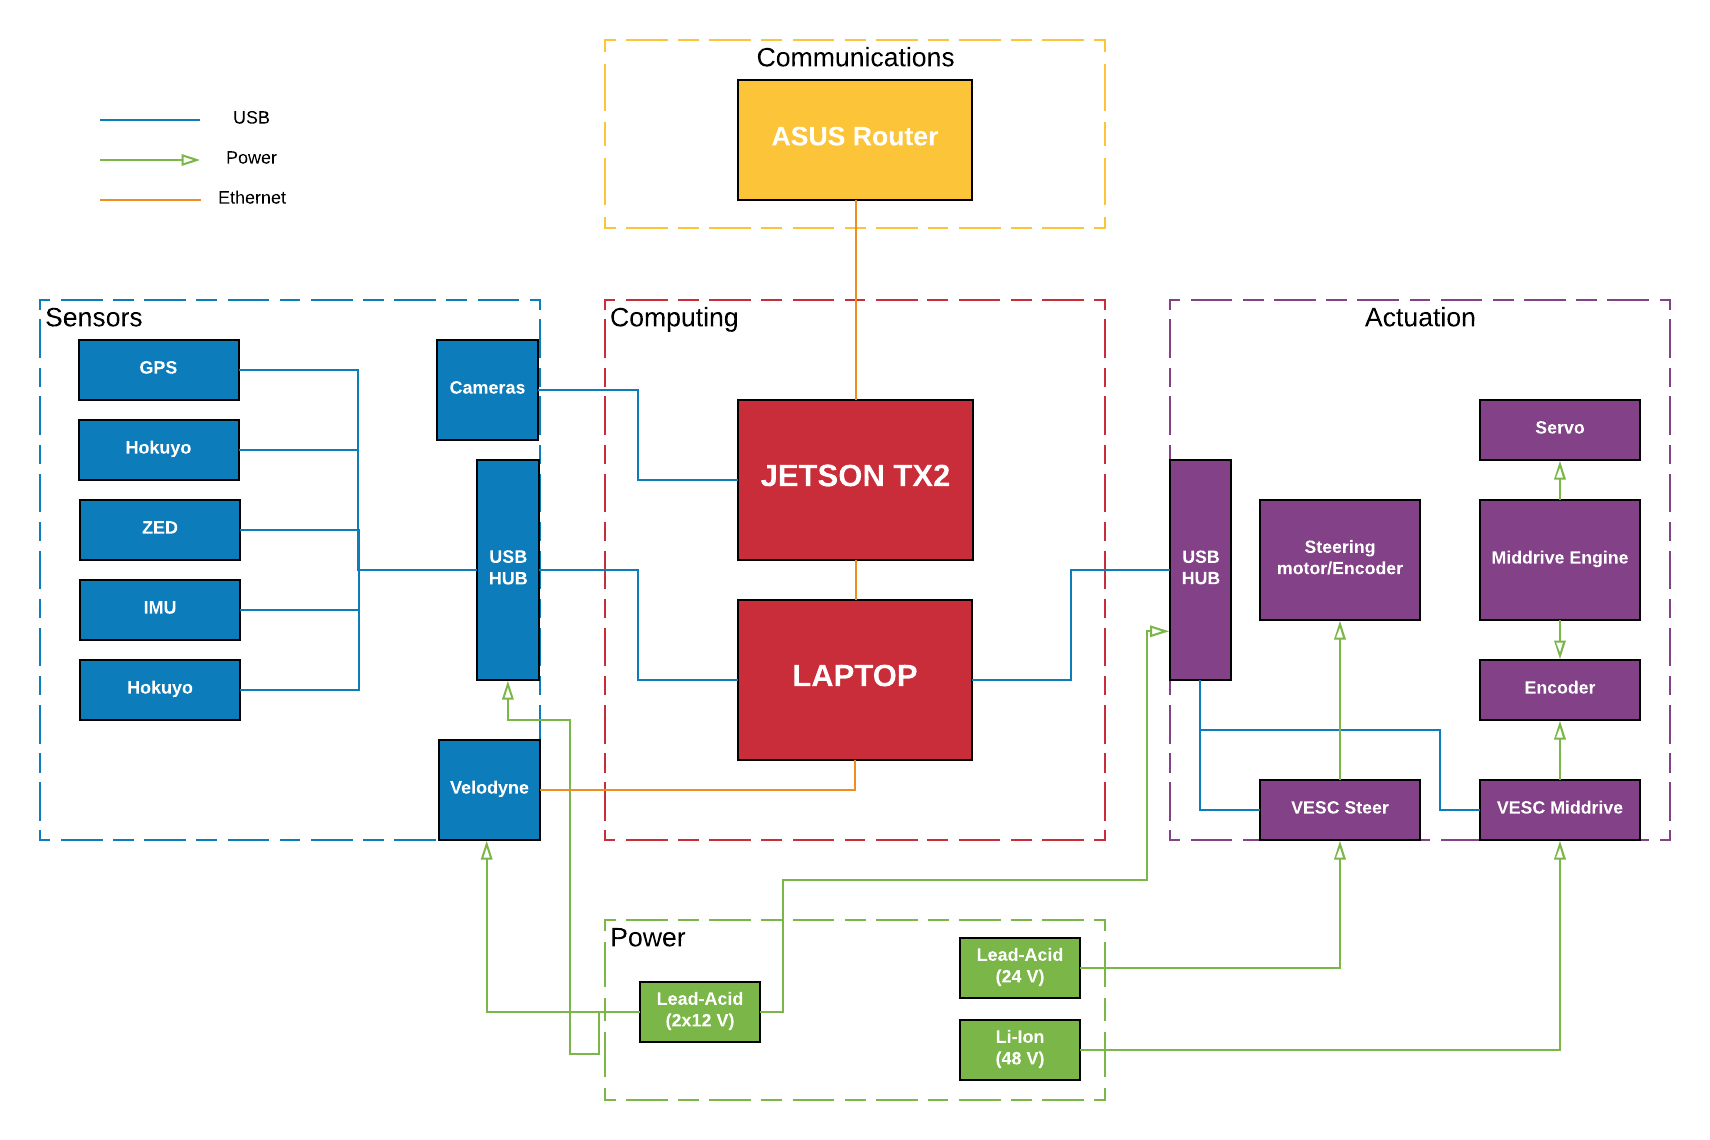
\includegraphics[width=1.8\linewidth, angle=-90]{pictures/05/pevsetup}}
  }
  \caption{PEV setup conceptual overview}
  \label{fig:pevsetup}
\end{figure}

\clearpage
The \textbf{master} of the ROS system is the laptop, but due to the wired communication, each computing unit can share information over the network. Both units are connected to the the router which can receive commands from smartphones and other devices.

Physically, all these components are housed on the front part, as it was mentioned before. Components are divided into 4 layers, and all sensors' cables are routed to their corresponding layer:
\begin{itemize}
  \item \textbf{First layer}: It houses the lead--acid batteries.

  \item \textbf{Second layer}: It houses an HVAC system that has not been mentioned because it is not in use, although it is on the road map.

  \item \textbf{Third layer}: Here, the USB hubs, ethernet switch and power boxes are located.

  \item \textbf{Fourth layer}: Places the Jetson TX2
\end{itemize}

\subsection{Control}

Control of the system is similar to the Nexus Robot, as speed commands come from 2 different sources: \textbf{Joystick} or \textbf{Navigation Stack}.

However, the control is more sophisticated, since the joystick can set the PEV in 3 different modes:
\begin{itemize}
  \item \textbf{Free mode}: In this state the PEV does not listen to any speed command and can move freely.

  \item \textbf{Autonomous mode}: While no speed commands are received, the servo brakes the wheel. When it receives input from either the joystick or the navigation stack, it starts moving autonomously.

  \item \textbf{Emergency Braking}: In this mode, the servo brakes the wheel and the PEV does not take any speed commands.
\end{itemize}

Besides this, speed commands are not sent directly to the VESC modules, a \textbf{speed multiplexor} is used instead. The workflow of the multiplexor is as follows:
\begin{itemize}
  \item \textbf{Inputs}: Navigation Stack and Joystick emit messages of the type \texttt{Twist} and \texttt{Joy}, so they are converted to \texttt{AckermannDriveStamped}.
  
  \item \textbf{Multiplexor}: Based on priority levels, the multiplexor outputs the speed command of the input with highest priority.

  \item \textbf{Ackermann to VESC node}: This node takes the speed command from the multiplexor, the joystick commands and the feedback from the VESC. If set in autonomous mode, it outputs one command to each of VESC modules, corrected with a PID controller.

  \item \textbf{VESC nodes}: Send the commands to the motors and feedback to the previous node in order to close the loop.
\end{itemize}

In \autoref{fig:pevcontrolsch}, an schematic of the whole control process is displayed.
\begin{figure}[htb]
  \centering
  \frame{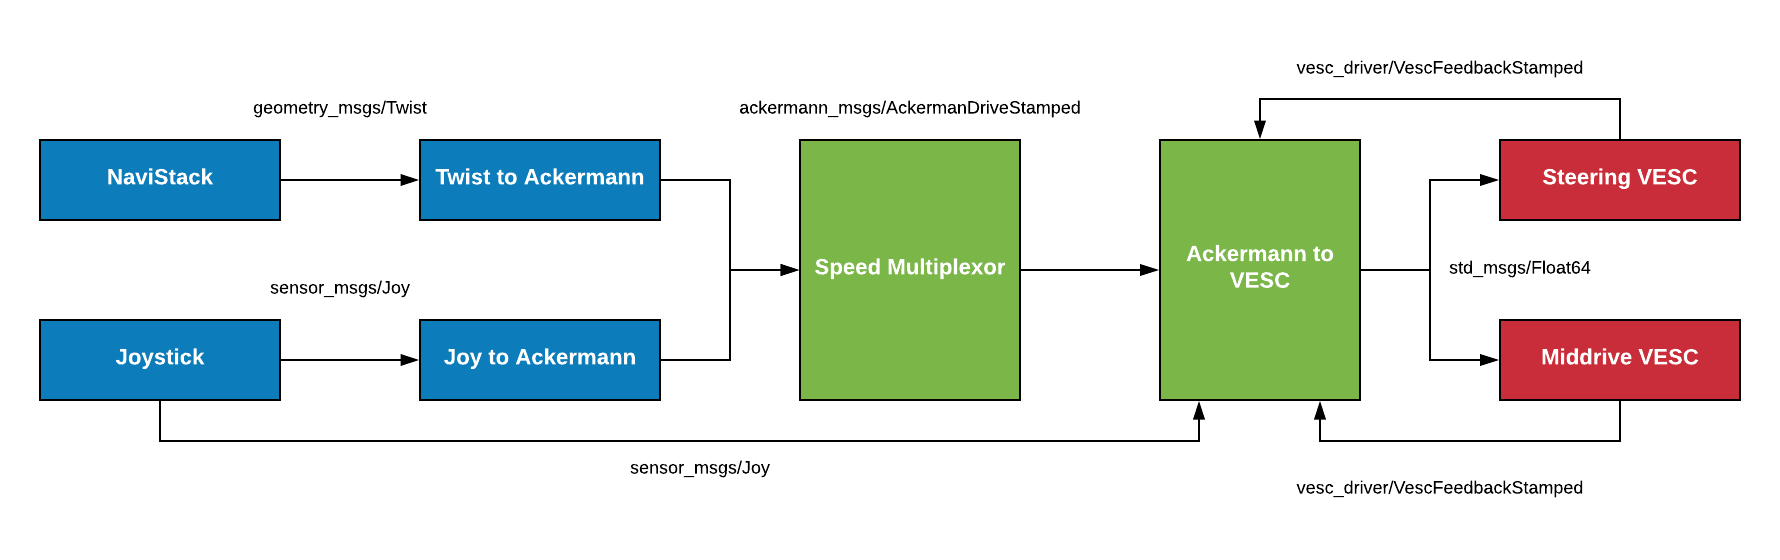
\includegraphics[width=\linewidth]{pictures/05/mux}}
  \caption{Schematic of PEV's control system}
  \label{fig:pevcontrolsch}
\end{figure}

\subsection{ROS package}

The ROS packages for the PEV is described in \autoref{tab:pevros}:
\begin{table}[h!]
  \centering
  \begin{tabular}{lp{8cm}}
    \hline
    \textbf{Package} & \textbf{Description} \\ \hline
    \textbf{firmware} & Code for the different controllers the PEV has (i.e, Arduino, Raspberry Pi) \\ \hline
    \textbf{pev\_autoware} & Necessary packages and messages from Autoware to run NDT mapping and localization \\ \hline
    \textbf{pev\_cmd\_mux} & Nodes of the multiplexor and its configuration files \\ \hline
    \textbf{pev\_description} & 3D model of the PEV in .urdf format \\ \hline
    \textbf{pev\_hardware\_rule} & Hardware rules of all the sensors of the PEV \\ \hline
    \textbf{pev\_mapping} & Configuration files for all the mapping algorithms \\ \hline
    \textbf{pev\_move} & Package to perform autonomous navigation. Contains nodes to send commands to motors, configuration files of localization algorithms and motion planners' parameters \\ \hline
    \textbf{pev\_msgs} & Custom services and messages for the PEV \\ \hline
    \textbf{pev\_octomap} & Package to perform 3D mapping. Deprecated \\ \hline
    \textbf{pev\_odom} & Nodes and configuration files to transform feedback from motors to odometry measurements \\ \hline
    \textbf{pev\_path\_server} & Nodes to save and load predefined paths for autonomous navigation \\ \hline
    \textbf{pev\_sensors} & Launch files  of all the sensors of the PEV \\ \hline
  \end{tabular}
  \caption{ROS packages for the PEV}
  \label{tab:pevros}
\end{table}

For SLAM, the most important packages are: \textbf{pev\_mapping}, \textbf{pev\_autoware}, \textbf{pev\_description}, \textbf{pev\_sensors} and \textbf{pev\_odom}.

\section{Indoor/Outdoor SLAM with PEV}

Three different scenarios were tested with the PEV: one indoor and 2 outdoor. The indoor scenario corresponds to \textbf{Media Lab's 6th floor}, where as the outdoor environments are \textbf{MIT Media Lab's courtyard} and \textbf{Taipei's Air Force Base}.

Because the data was collected in such diverse areas, the 4 SLAM algorithms have been employed (not all in all cases). Recalling from (\autoref{ch:slam}) those algorithms are: \textbf{Gmapping}, \textbf{Hector SLAM}, \textbf{Google's Cartographer} and \textbf{Autoware}.

\subsection{Media Lab 6th floor}
The 6th floor of the Media Lab is very well-known in the Boston area for its impressive views and it is often used for all kinds of conferences and venues. It is a relatively large open--space (800 m\textsuperscript{2}), therefore it is ideal to test the PEV when new features are developed or when the weather conditions do not allow for outdoor testing.

\parunder{Gmapping on 6th floor}
The first algortihm to be tested is the Gmapping algorithm. As it was done with the Nexus robot, several parameters were varied to find the optimal configuration (\autoref{tab:pevgmapping6}):
\begin{table}[h]
  \centering
  \begin{tabular}{lc}
  \hline
  \textbf{Parameter} & \textbf{Range} \\ \hline
  Default & - \\ \hline
  Linear update rate & {[}0.1-1.0{]} \\ \hline
  Angular update rate & {[}0.1-1.0{]} \\ \hline
  Iterations for the scanmatcher & {[}0-10{]} \\ \hline
  \end{tabular}
  \caption{Tests with Gmapping in the 6th floor}
  \label{tab:pevgmapping6}
\end{table}

The results for Gmapping are shown in \autoref{fig:pevgm6var}. As it can be seen, there is not much difference in any of the cases studied.
It is true that in the default case, edges of the map appear to be 'blurrier' but this issue is mitigated by applying the same reasoning as with the Nexus Robot. 
\begin{figure}[htb]
  \centering
  \subfloat[Default values]{\frame{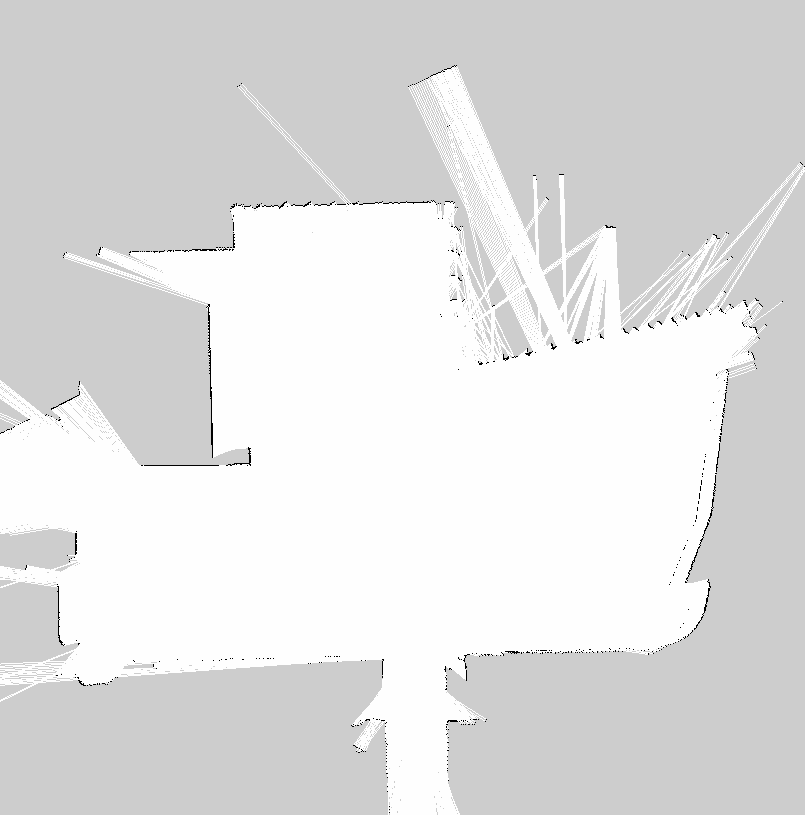
\includegraphics[width=.45\linewidth]{pictures/05/6_floor/gmapping/default}}} \quad
  \subfloat[Linear update of 0.1 m]{\frame{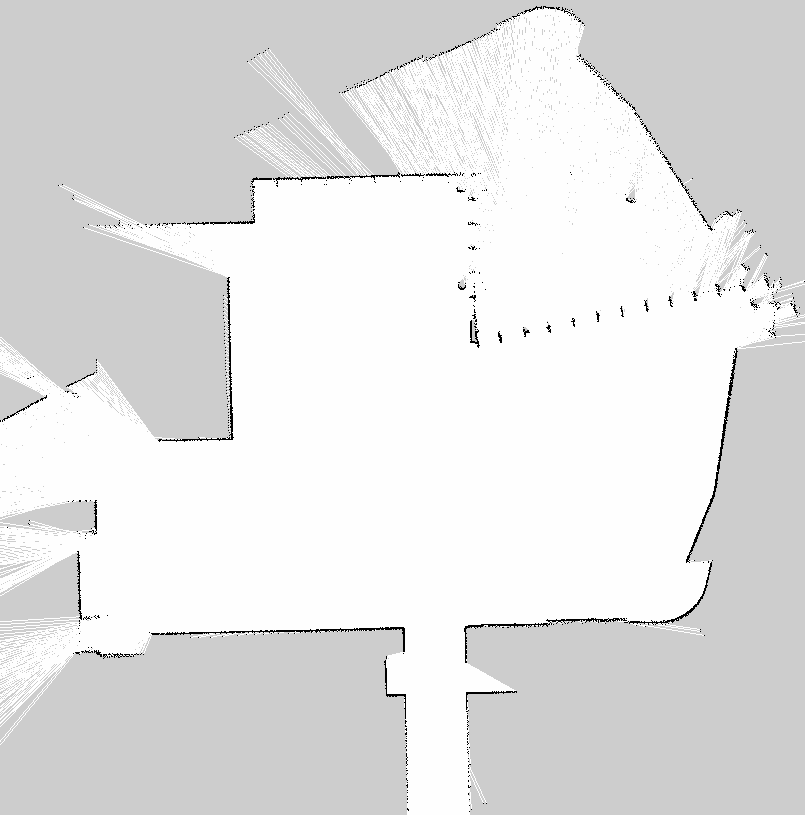
\includegraphics[width=.45\linewidth]{pictures/05/6_floor/gmapping/linear010}}} \\
  \subfloat[Angular update of 0.1 rad]{\frame{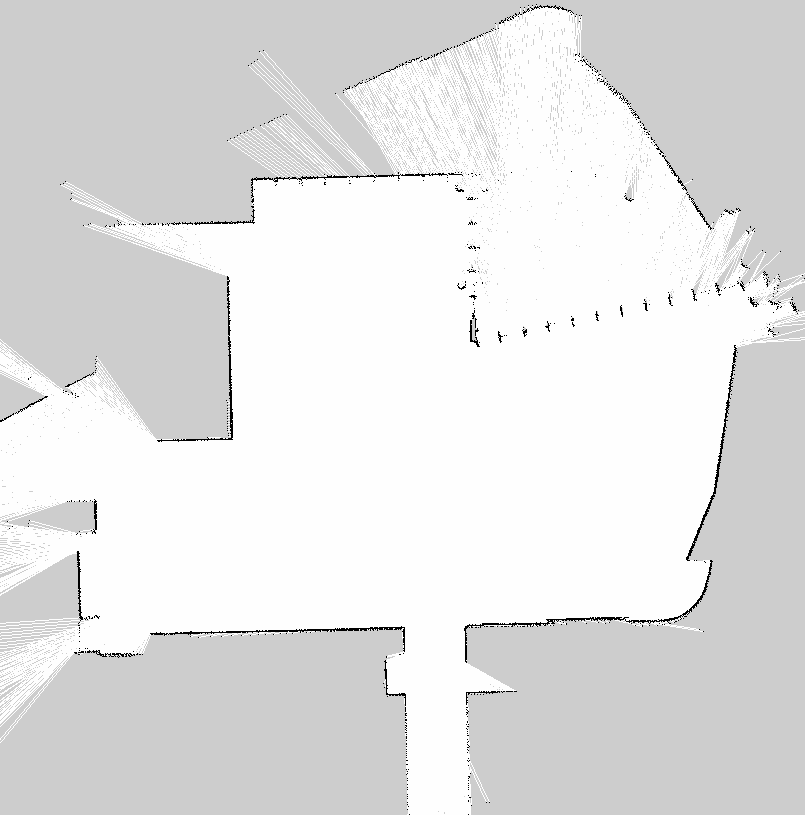
\includegraphics[width=.45\linewidth]{pictures/05/6_floor/gmapping/angular010}}} \quad 
  \subfloat[10 iterations]{\frame{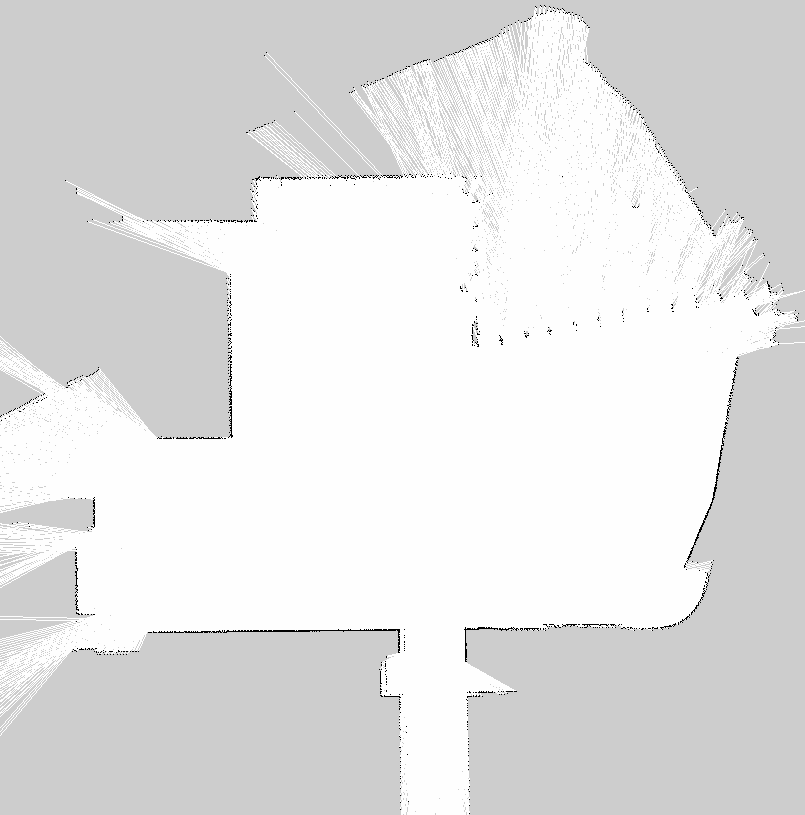
\includegraphics[width=.45\linewidth]{pictures/05/6_floor/gmapping/iteration10}}} \\  
  \caption{Gmapping on the 6th floor}
  \label{fig:pevgm6var}
\end{figure}

Generally speaking, the quality of the maps obtained is more than acceptable for autonomous navigation with only a little adjustment to be made on the upper right area (edges are not detected because doors are made of glass).

As a matter of fact, the odometry data (which is necessary to run the Gmapping algorithm) is not provided by the wheel and motor encoders, but by a ROS library that estimates odometry from laser \citepev{Jaimez2016}. As it can be seen, the quality of the estimation is good enough, since results are satisfactory.

\parunder{Hector on 6th floor} Recalling from previous chapters, odometry is optional in Hector SLAM, and generally there is not much difference. For that reason, results are provided without using it. \autoref{tab:pevhector6} summarizes the variations tested:
\begin{table}[h!]
  \centering
  \begin{tabular}{lc}
  \hline
  \textbf{Parameter} & \textbf{Range} \\ \hline
  Default & - \\ \hline
  Linear update rate & {[}0.1-1.0{]} \\ \hline
  Angular update rate & {[}0.1-1.0{]} \\ \hline
  Map resolution & 2 \& 3 \\ \hline
  \end{tabular}
  \caption{Tests with Hector in the 6th floor}
  \label{tab:pevhector6}
\end{table}

The results (\autoref{fig:pevhe6var}), show that there is no appreciable difference in any of the cases tested. However, the accuracy is slightly better than Gmapping, as edges are sharper and there is less diffusion.
\begin{figure}[htb]
  \centering
  \subfloat[Default values]{\frame{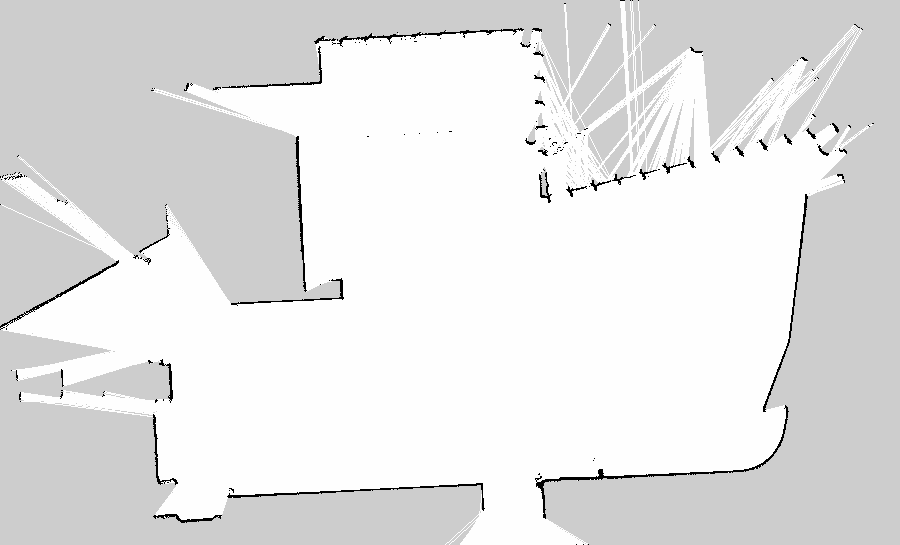
\includegraphics[width=.45\linewidth]{pictures/05/6_floor/hector/nodommulti3default}}} \quad
  \subfloat[Default values]{\frame{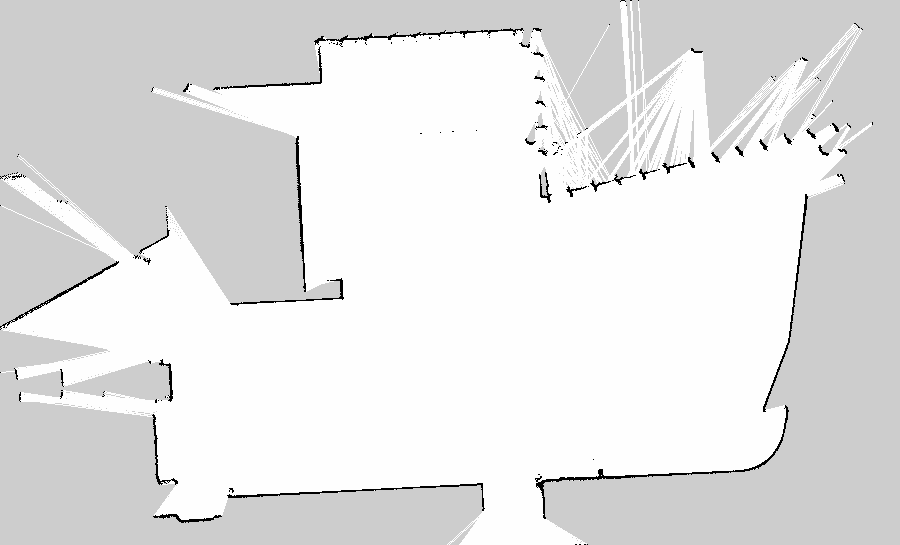
\includegraphics[width=.45\linewidth]{pictures/05/6_floor/hector/nodommulti2default}}} \\
  \subfloat[Linear update of 0.1 m]{\frame{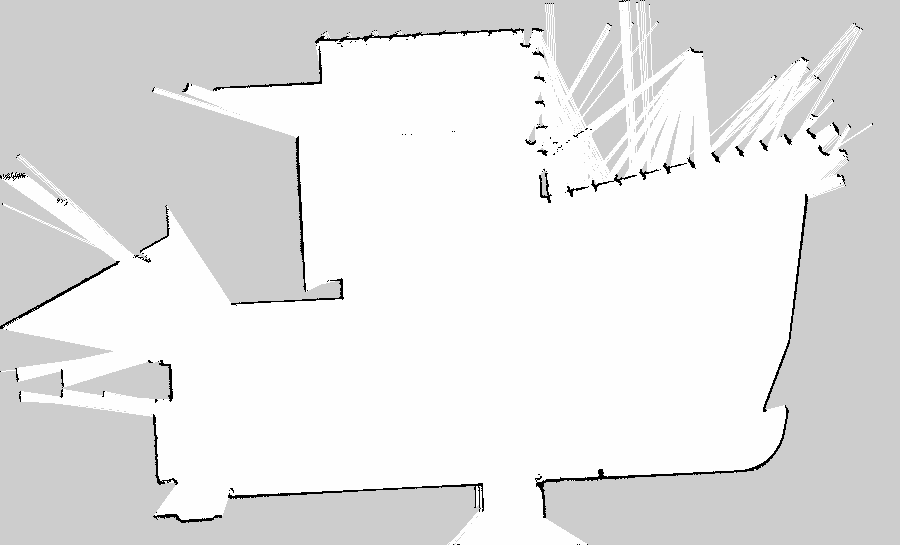
\includegraphics[width=.45\linewidth]{pictures/05/6_floor/hector/nodommulti3linear020}}} \quad 
  \subfloat[Linear update of 0.1 m]{\frame{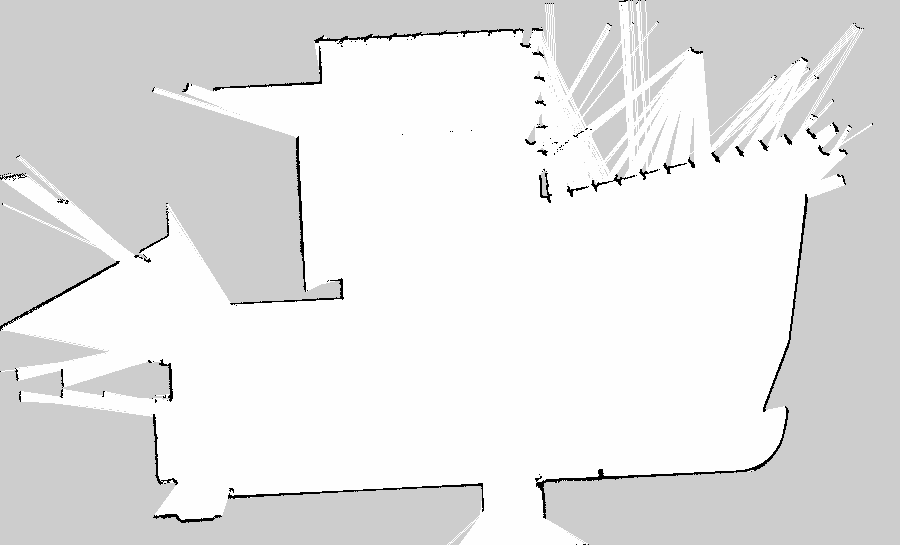
\includegraphics[width=.45\linewidth]{pictures/05/6_floor/hector/nodommulti2linear020}}} \\  
  \subfloat[Angular update of 0.4 rad]{\frame{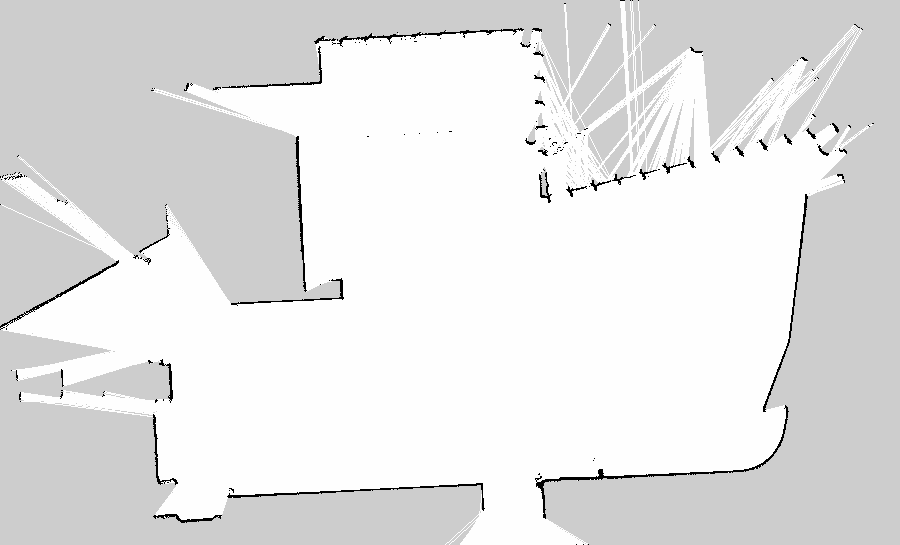
\includegraphics[width=.45\linewidth]{pictures/05/6_floor/hector/nodommulti3angular040}}} \quad 
  \subfloat[Angular update of 0.4 rad]{\frame{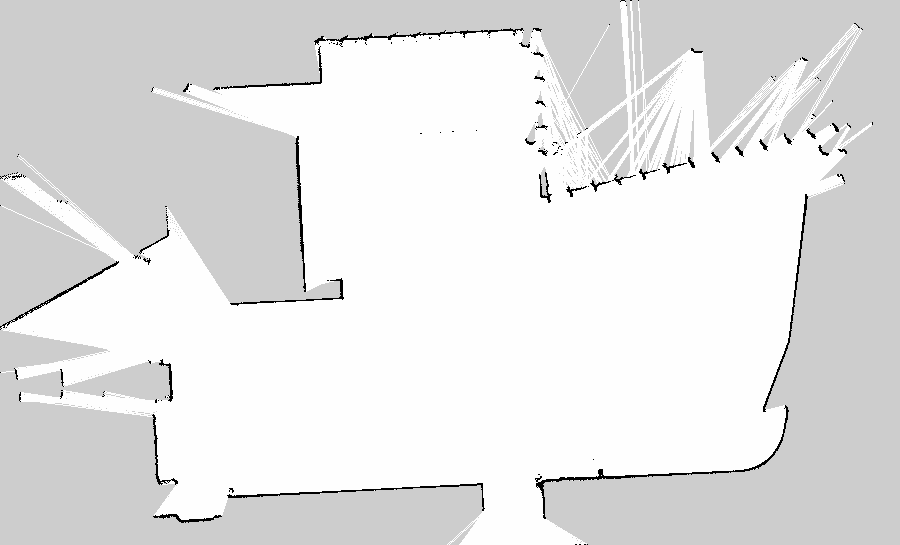
\includegraphics[width=.45\linewidth]{pictures/05/6_floor/hector/nodommulti2angular040}}} \\ 
  \caption[Hector on the 6th floor]{Hector on the 6th floor. Map resolution 3 (left) and 2 (right)}
  \label{fig:pevhe6var}
\end{figure}

\parunder{Cartographer on 6th floor} Tuning Cartographer is not as straight forward as tuning Hector SLAM or Gmapping. The number of parameters is much larger and not every parameter is documented on the API. Furthermore, Cartographer can run with or without odometry and IMU when mapping in 2 dimensions.

The parameters that have been tuned are shown in \autoref{tab:pevcarto6}. The default parameters are obtained from the \texttt{backpack\_2d.lua} file provided by cartographer. Results with IMU are shown on \autoref{fig:pevcarto6imu} and without it on \autoref{fig:pevcarto6noimu}.
\begin{table}[h!]
  \centering
  \begin{tabular}{lc}
  \hline
  \textbf{Parameter} & \textbf{Range} \\ \hline
  Default & - \\ \hline
  Accumulated range data & {[}1-10{]} \\ \hline
  Lidar type & {[}Velodyne and Hokuyo{]} \\ \hline
  \end{tabular}
  \caption{Tests with Cartographer in the 6th floor}
  \label{tab:pevcarto6}
\end{table}

\begin{figure}[t!]
  \centering
  \subfloat[Default]{\frame{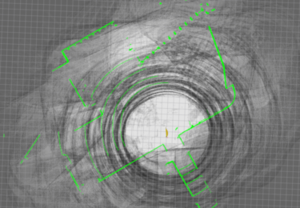
\includegraphics[width=.45\linewidth]{pictures/05/6_floor/cartographer/imuacc10}}} \quad
  \subfloat[Accumulated data 5]{\frame{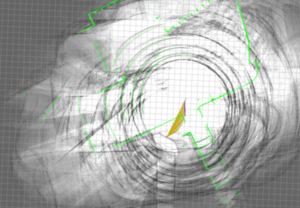
\includegraphics[width=.45\linewidth]{pictures/05/6_floor/cartographer/imuacc5}}} \\
  \subfloat[Accumulated data 1]{\frame{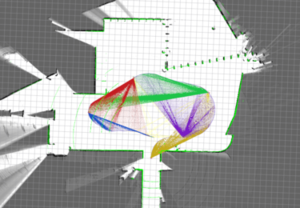
\includegraphics[width=.45\linewidth]{pictures/05/6_floor/cartographer/imuacc1}}} \quad 
  \subfloat[Using Hokuyo Lidar]{\frame{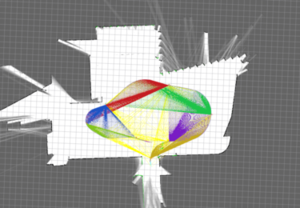
\includegraphics[width=.45\linewidth]{pictures/05/6_floor/cartographer/imu2d}}} \\  
  \caption{Cartographer on the 6th floor (with IMU)}
  \label{fig:pevcarto6imu}
\end{figure}

\begin{figure}[h!]
  \centering
  \subfloat[Default]{\frame{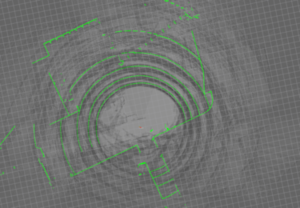
\includegraphics[width=.45\linewidth]{pictures/05/6_floor/cartographer/noimuacc10}}} \quad
  \subfloat[Accumulated data 5]{\frame{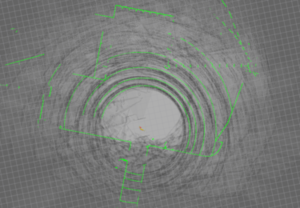
\includegraphics[width=.45\linewidth]{pictures/05/6_floor/cartographer/noimuacc5}}} \\
  \subfloat[Accumulated data 1]{\frame{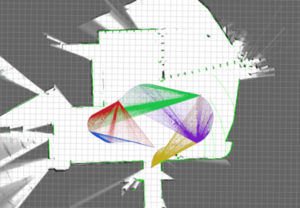
\includegraphics[width=.45\linewidth]{pictures/05/6_floor/cartographer/noimuacc1}}} \quad 
  \subfloat[Using Hokuyo Lidar]{\frame{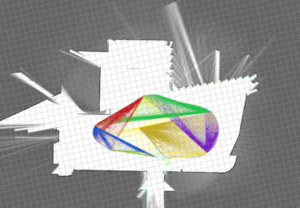
\includegraphics[width=.45\linewidth]{pictures/05/6_floor/cartographer/noimu2d}}} \\  
  \caption{Cartographer on the 6th floor (without IMU)}
  \label{fig:pevcarto6noimu}
\end{figure}

First thing to notice is that when accumulated laser data grows, the SLAM process results in incomprehensible maps. The difference of using the 3D Velodyne lidar or the 2D Hokuyo is the higer range of the former, which results in more features mapped. Another aspect to point out is that there is virtually no difference between using IMU or relying solely on the scanmatcher. Finally, when using the 2D Lidar, it can be seen that the results are as good as with the previous approaches.

It can be concluded that for this environment Cartographer's theoretical advantage over Gmapping and Hector is unappreciable.

\subsection{MIT Media Lab's Courtyard}
On the back door of the Media Lab there is an extense courtyard that serves as an outdoor testing site for the PEV (\autoref{fig:courtyardsat}). The area is much larger than the previous studied environments (2000 m\textsuperscript{2}), although it is 'closed' in the sense that it does not communicate with the street directly. Therefore, it serves as a middleground between indoor and pure outdoor areas.
\begin{figure}[h!]
  \centering
  \frame{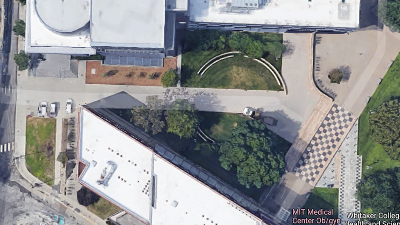
\includegraphics[width=\linewidth]{pictures/05/courtyardsat}}
  \caption{Satellite image of the courtyard}
  \label{fig:courtyardsat}
\end{figure}

\parunder{Gmapping on courtyard} The parameters that were varied in the courtyard are summarized on \autoref{tab:pevgmappingcou}, and various results can be seen on \autoref{fig:pevgmcouvar}.
\begin{table}[h]
  \centering
  \begin{tabular}{lc}
    \hline
    \textbf{Parameter} & \textbf{Range} \\ \hline
    Default & - \\ \hline
    Linear update rate & {[}0.1-0.5{]} \\ \hline
    Angular update rate & {[}0.1-0.5{]} \\ \hline
    Iterations for the scanmatcher & {[}0-10{]} \\ \hline
  \end{tabular}
  \caption{Tests with Gmapping on the courtyard}
  \label{tab:pevgmappingcou}
\end{table}

\begin{figure}[t]
  \centering
  \subfloat[Default values]{\frame{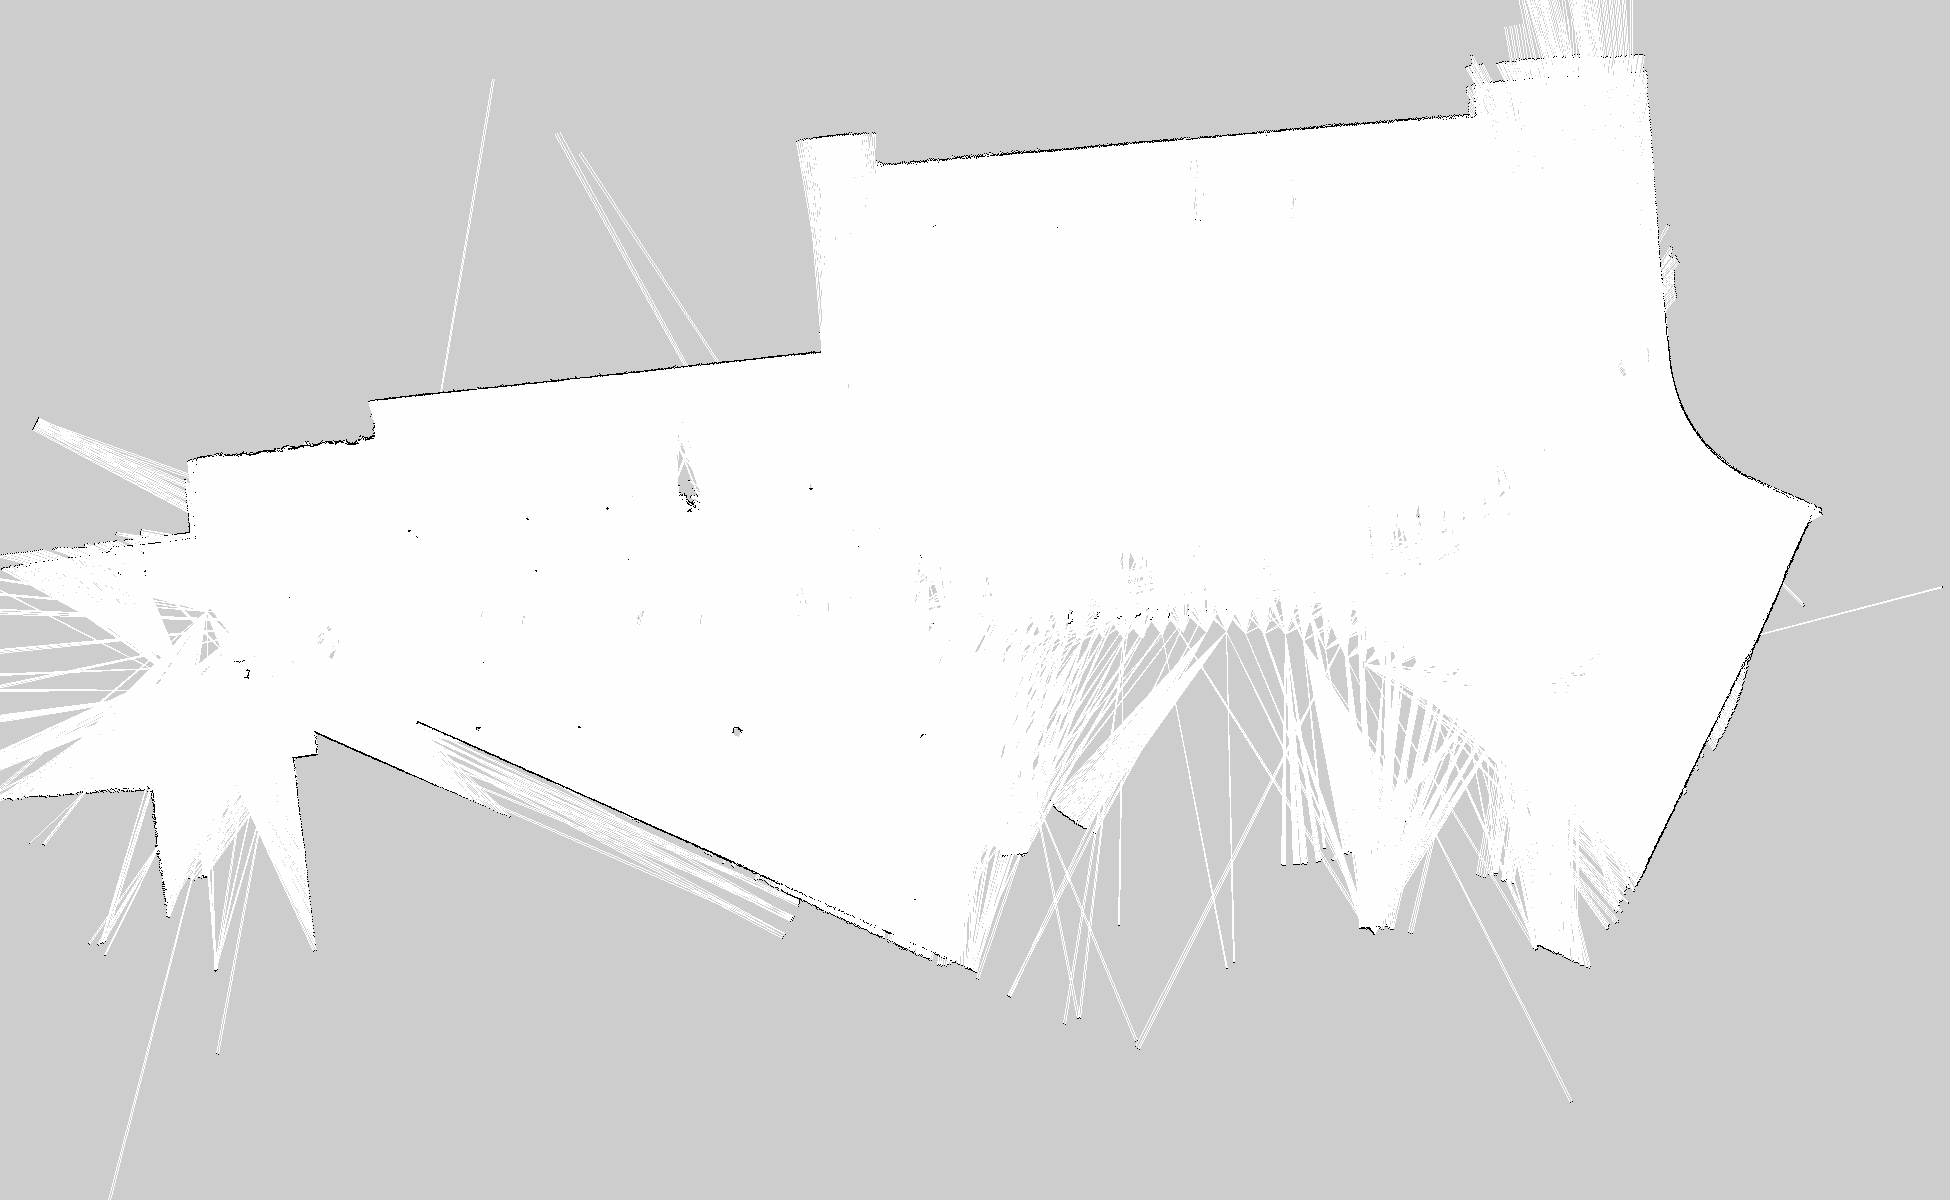
\includegraphics[width=.45\linewidth]{pictures/05/courtyard/gmapping/default30m}}} \quad
  \subfloat[Linear update of 0.1 m]{\frame{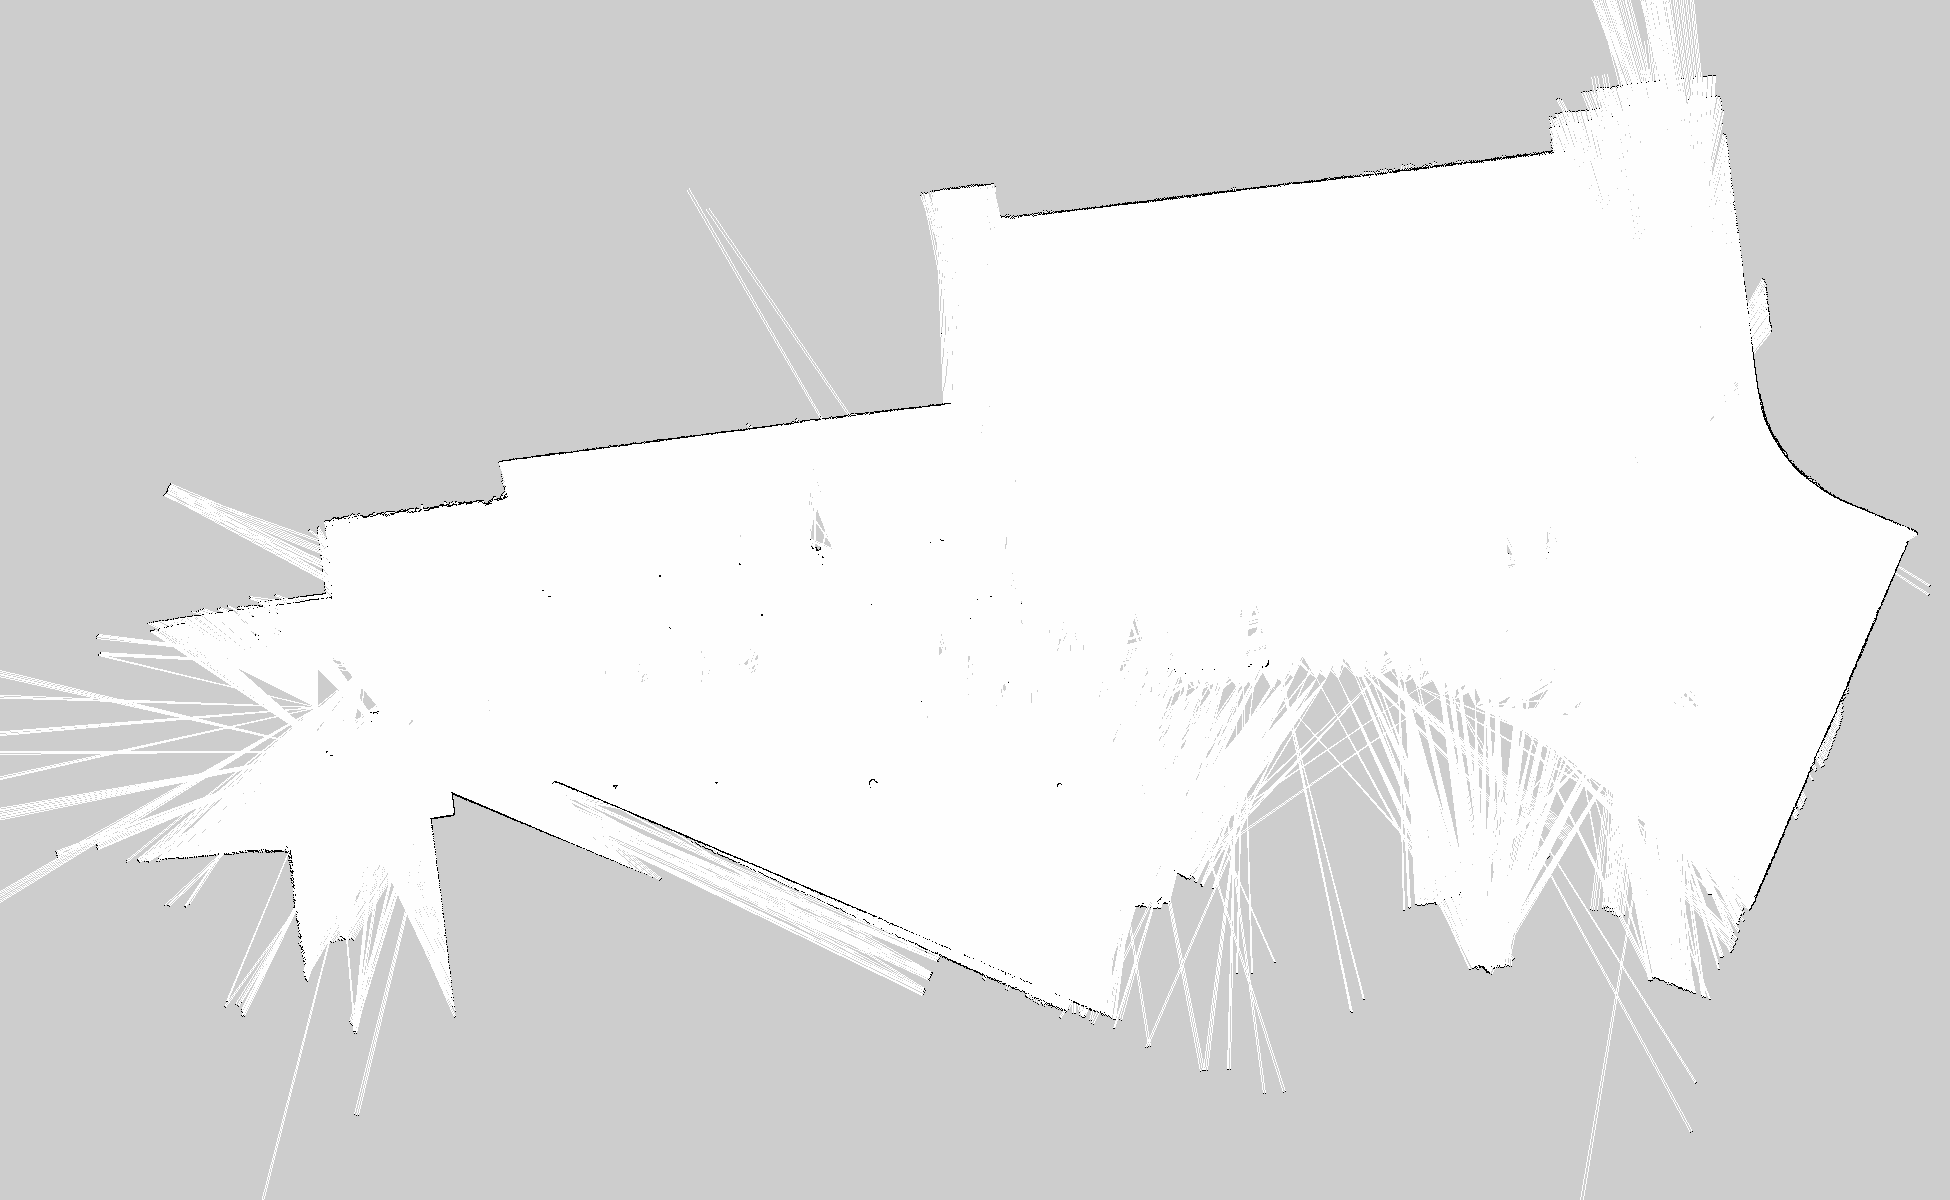
\includegraphics[width=.45\linewidth]{pictures/05/courtyard/gmapping/linear01030m}}} \\
  \subfloat[Angular update of 0.2 rad]{\frame{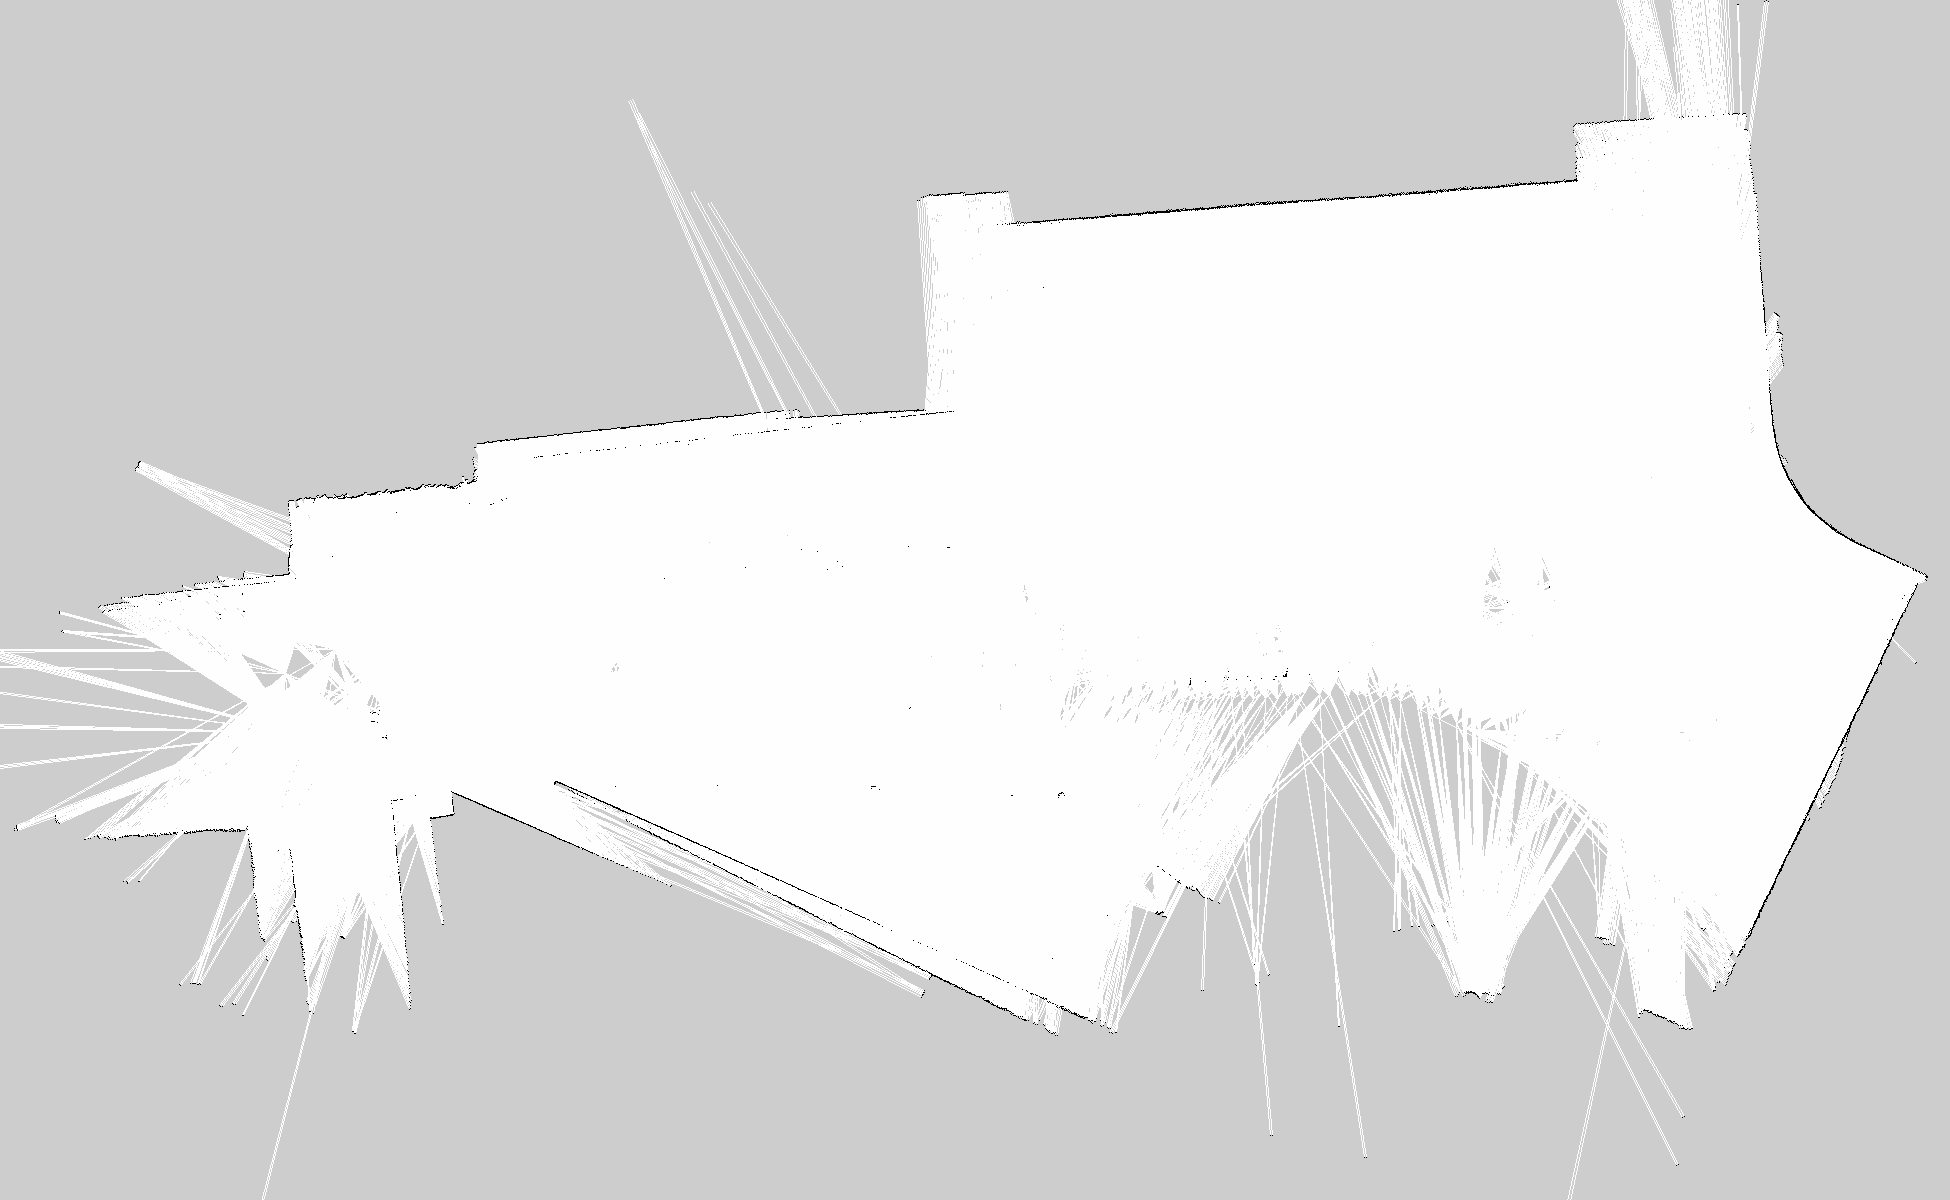
\includegraphics[width=.45\linewidth]{pictures/05/courtyard/gmapping/angular02030m}}} \quad 
  \subfloat[10 iterations]{\frame{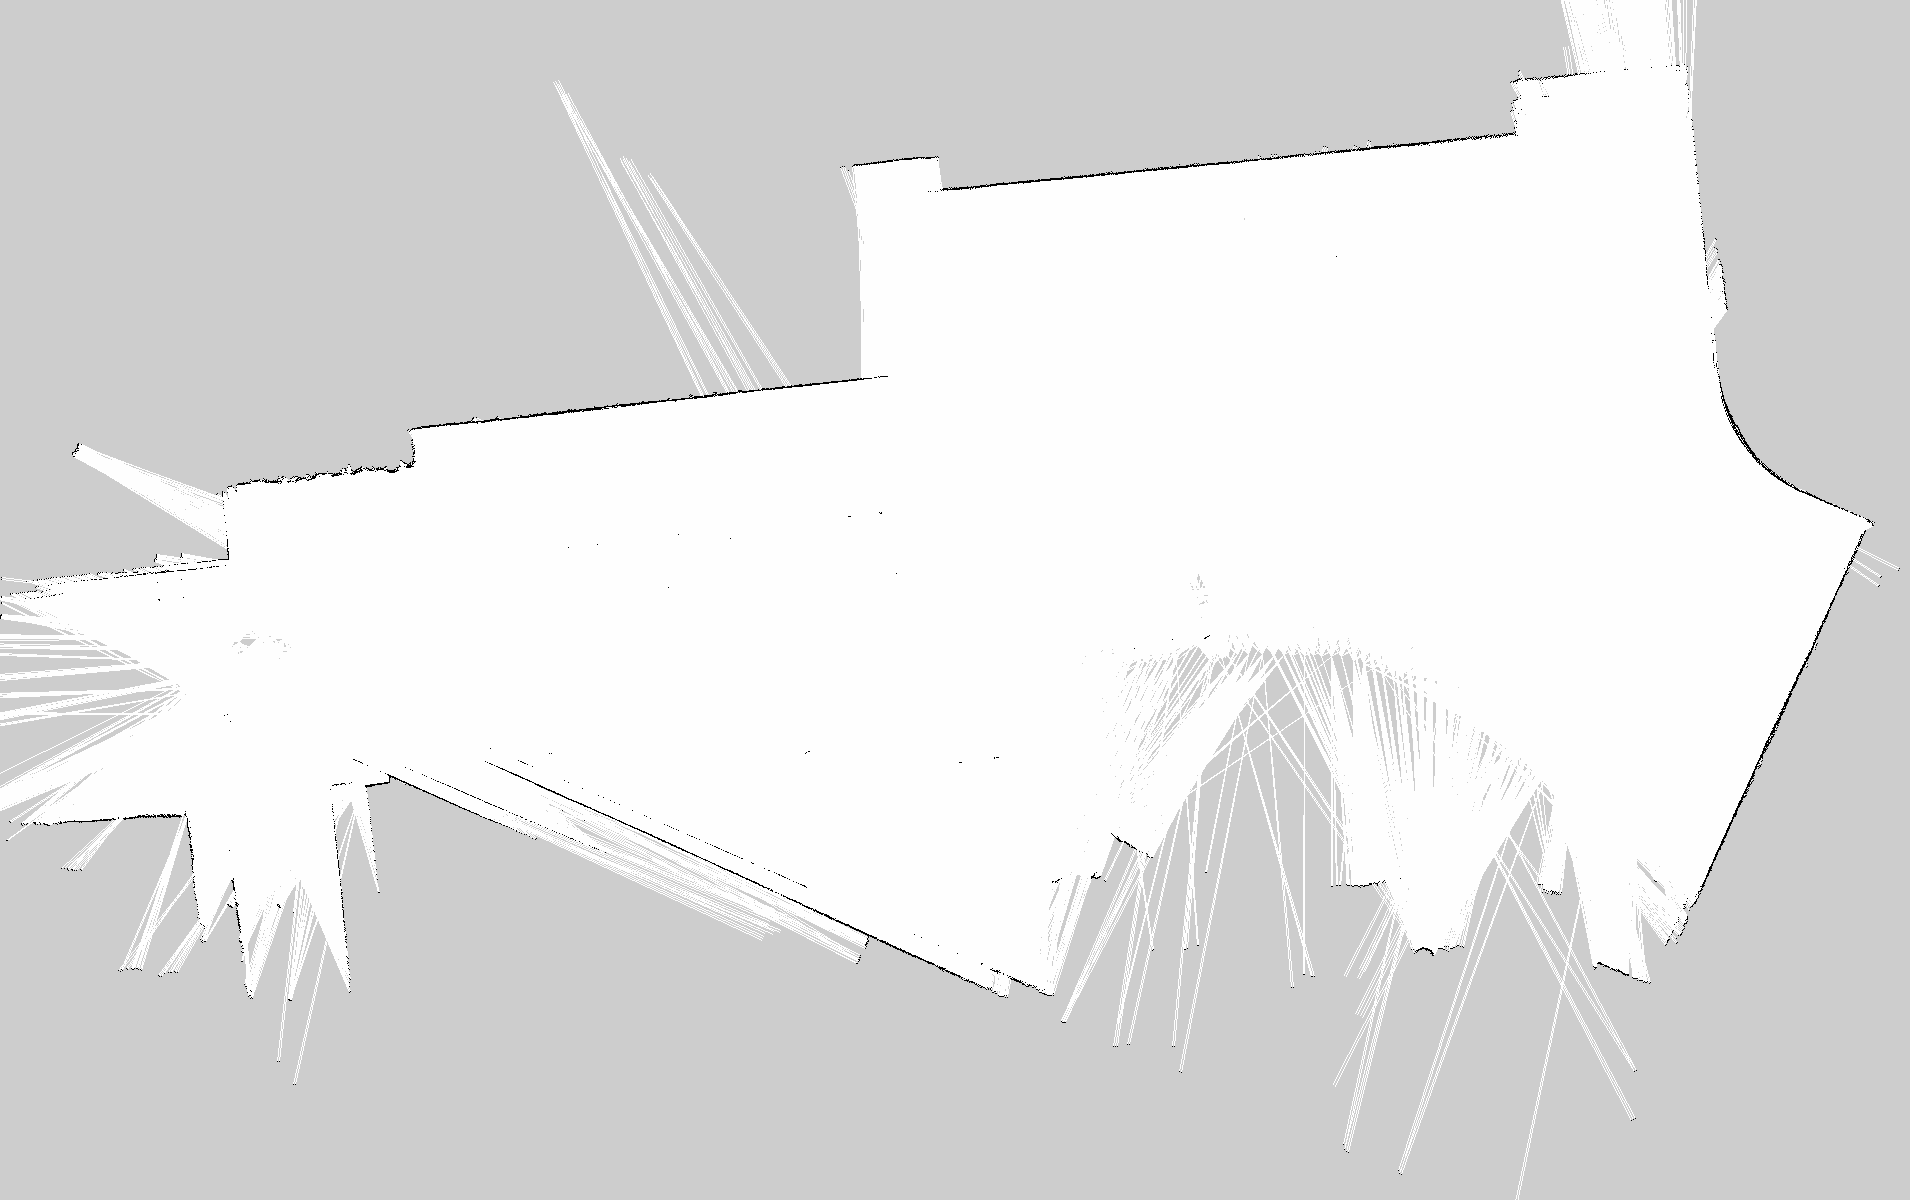
\includegraphics[width=.45\linewidth]{pictures/05/courtyard/gmapping/iteration1030m}}} \\  
  \caption{Gmapping on the courtyard}
  \label{fig:pevgmcouvar}
\end{figure}

None of the configurations tried througout the experiments improved the quality of the above shown maps. Although quality is not acceptable for autonomous navigation, the main shaoe of the area is conserved. The biggest gap that appears on the lower end of the map is due to the 30 m limit of the Hokuyo lidar.

With some manual adjustments, however, these maps could be utilized for localization.

\parunder{Hector on courtyard} With regards to employing Hector SLAM on the courtyard, \autoref{tab:pevhectorcou} gathers the variations tested.
\begin{table}[h!]
  \centering
  \begin{tabular}{lc}
    \hline
    \textbf{Parameter} & \textbf{Range} \\ \hline
    Default & - \\ \hline
    Linear update rate & {[}0.1-1.0{]} \\ \hline
    Angular update rate & {[}0.1-1.0{]} \\ \hline
    Map resolution & 2 \& 3 \\ \hline
  \end{tabular}
  \caption{Tests with Hector on the courtyard}
  \label{tab:pevhectorcou}
\end{table}

As it can be seen on \autoref{fig:pevhecouvar}, none of the results for the Hector SLAM is acceptable, nor it could be manually adjusted. The reason why this might be ocurring is that Hector SLAM relies on the scan matcher but the central area of the courtyard is too wide for the 30 m laser scanner to find features. Therefore, the matching operation fails, leading to bad results. To improve this, it would be necssary a longer range sensor.

\begin{figure}[t!]
  \centering
  \subfloat[Default values]{\frame{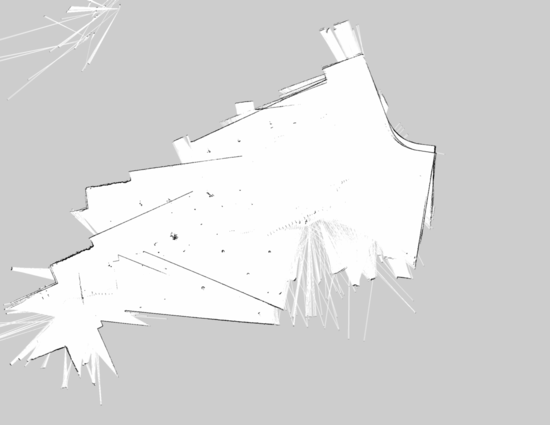
\includegraphics[width=.45\linewidth]{pictures/05/courtyard/hector/odommulti3default}}} \quad
  \subfloat[Default values]{\frame{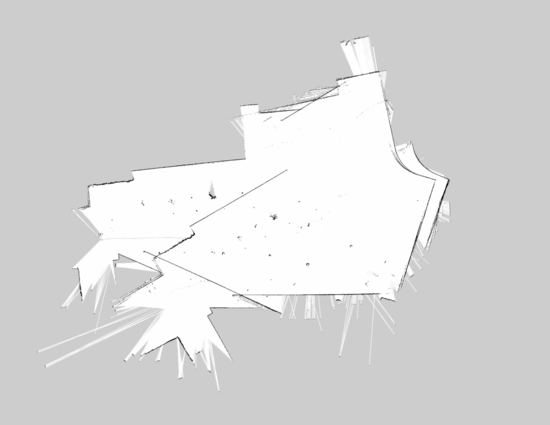
\includegraphics[width=.45\linewidth]{pictures/05/courtyard/hector/odommulti2default}}} \\
  \subfloat[Linear update of 0.2 m]{\frame{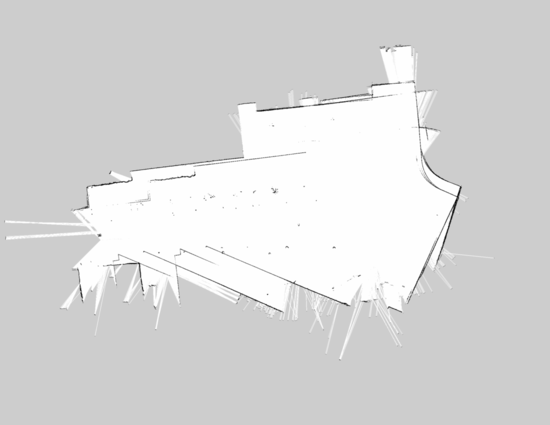
\includegraphics[width=.45\linewidth]{pictures/05/courtyard/hector/odommulti3linear020}}} \quad 
  \subfloat[Linear update of 0.2 m]{\frame{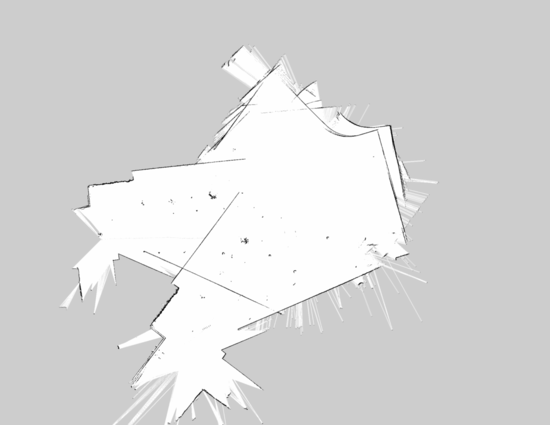
\includegraphics[width=.45\linewidth]{pictures/05/courtyard/hector/odommulti2linear020}}} \\  
  \subfloat[Angular update of 0.2 rad]{\frame{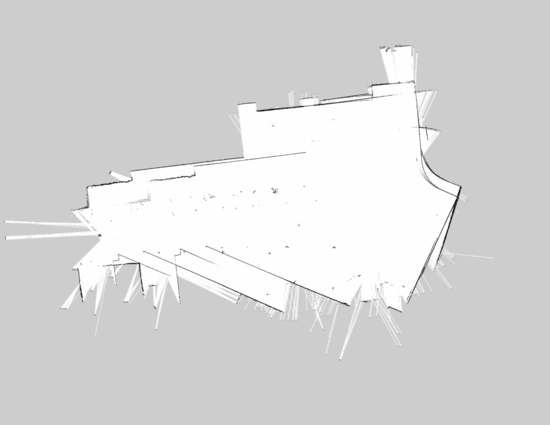
\includegraphics[width=.45\linewidth]{pictures/05/courtyard/hector/odommulti3angular020}}} \quad 
  \subfloat[Angular update of 0.4 rad]{\frame{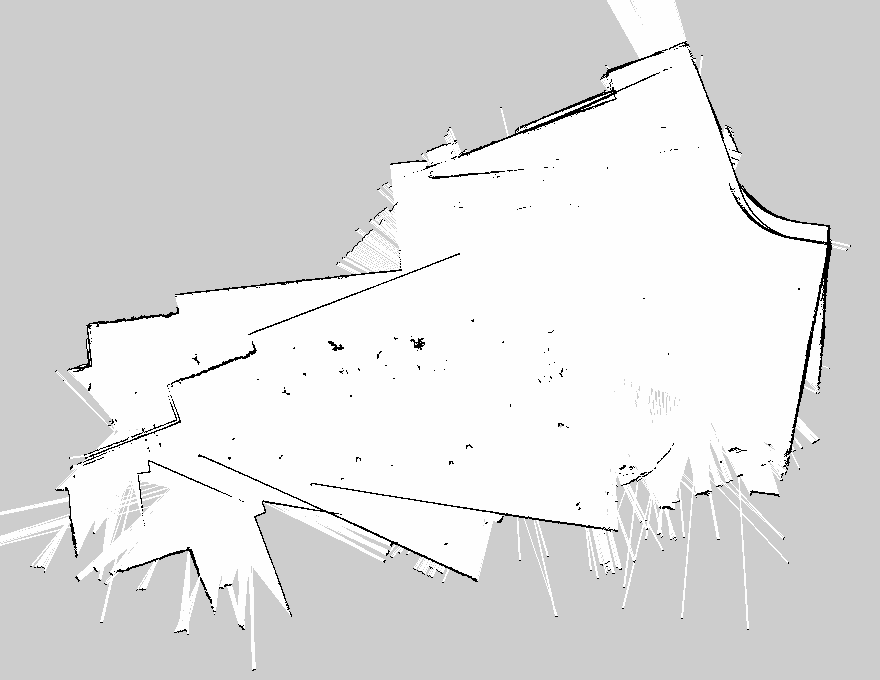
\includegraphics[width=.45\linewidth]{pictures/05/courtyard/hector/odommulti2angular020}}} \\ 
  \caption[Hector on the courtyard]{Hector on the courtyard. Map resolution 3 (left) and 2 (right)}
  \label{fig:pevhecouvar}
\end{figure}

\parunder{Cartographer on courtyard} With regards to Cartographer, the configurations tested can be checked on \autoref{tab:pevcartocou}. Results with IMU and without are displayed on \autoref{fig:pevcartocouimu} and \autoref{fig:pevcartocounoimu}.
\begin{table}[t!]
  \centering
  \begin{tabular}{lc}
    \hline
    \textbf{Parameter} & \textbf{Range} \\ \hline
    Default & - \\ \hline
    Max z laser & {[}0.5-2.0{]} \\ \hline
    Min z laser & {[}-0.5-1.0{]} \\ \hline
    Translational weight & {[}2-200{]} \\ \hline
    Rotational weight & {[}5-500{]} \\ \hline
    Lidar type & {[}Velodyne and Hokuyo{]} \\ \hline
  \end{tabular}
  \caption{Tests with Cartographer on the courtyard}
  \label{tab:pevcartocou}
\end{table}

\begin{figure}[t!]
  \centering
  \subfloat[Default]{\frame{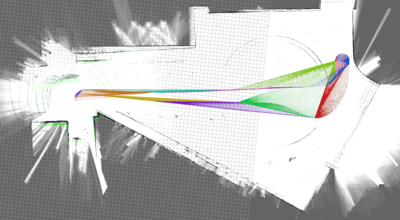
\includegraphics[width=.45\linewidth]{pictures/05/courtyard/cartographer/imudef}}} \quad
  \subfloat[Min max z: 0.5-1.5 m]{\frame{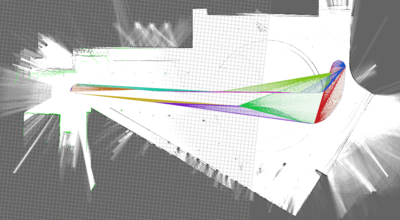
\includegraphics[width=.45\linewidth]{pictures/05/courtyard/cartographer/imu0515}} \label{fig:pevcartocouimu25}} \\
  \subfloat[Trans/Rot. weights: 200/500]{\frame{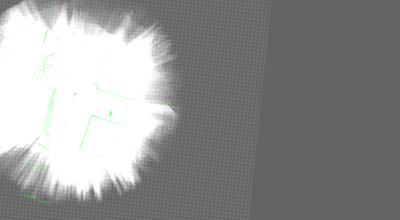
\includegraphics[width=.45\linewidth]{pictures/05/courtyard/cartographer/imue2}}} \quad 
  \subfloat[Using Hokuyo Lidar]{\frame{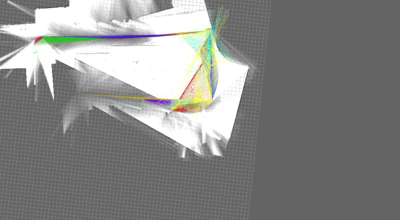
\includegraphics[width=.45\linewidth]{pictures/05/courtyard/cartographer/imu2d}}} \\  
  \caption{Cartographer on the courtyard (with IMU)}
  \label{fig:pevcartocouimu}
\end{figure}

\begin{figure}[ht]
  \centering
  \subfloat[Default]{\frame{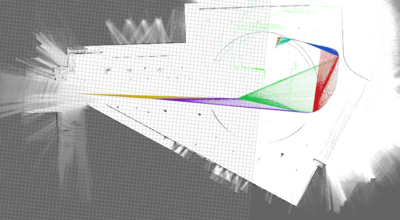
\includegraphics[width=.45\linewidth]{pictures/05/courtyard/cartographer/noimudef}}} \quad
  \subfloat[Min max z: 0.5-1.5 m]{\frame{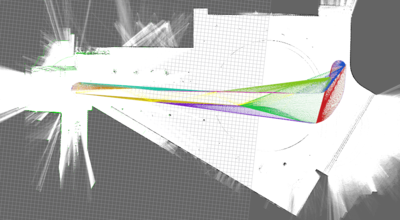
\includegraphics[width=.45\linewidth]{pictures/05/courtyard/cartographer/noimu0515}} \label{fig:pevcartocounoimu25}} \\
  \subfloat[Trans/Rot. weights: 200/500]{\frame{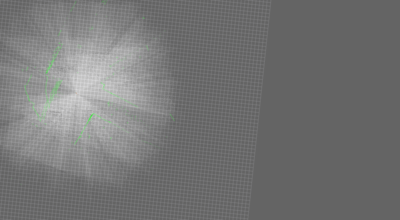
\includegraphics[width=.45\linewidth]{pictures/05/courtyard/cartographer/noimue2}}} \quad 
  \subfloat[Using Hokuyo Lidar]{\frame{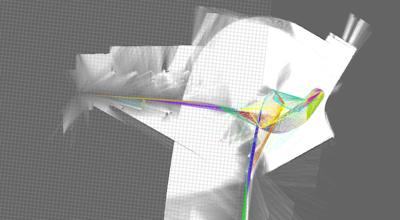
\includegraphics[width=.45\linewidth]{pictures/05/courtyard/cartographer/noimu2d}}} \\  
  \caption{Cartographer on the courtyard(without IMU)}
  \label{fig:pevcartocounoimu}
\end{figure}

The configuration for the best result achieved in the 6th floor does not provide a perfect solution but it can serve as a starting point. The parameters that have the more direct influence on the quality of the map are the translational and rotational weights. On \autoref{fig:pevcartocouimu}\protect\subref{fig:pevcartocouimu25} and \autoref{fig:pevcartocounoimu}\protect\subref{fig:pevcartocounoimu25} these weights were set to 2 and 5, and yield very good results. Adding to that, the range of 0.5-1.5 m improves the speed of the computation and results in the most accurate maps for each case.

\clearpage
In these tests the difference of using IMU and not using it is more notorius. However, what seems counterintuitive is that the best results are achieved when IMU is not considered. A possible explanation could be miscalibration of inertial sensors, but the lidar-only approach still provides more consistent results when using data from other days.

\parunder{NDT on courtyard} NDT mapping does not allow to change any of its parameters, except for the use of IMU. The processing of the file took around 15 minutes and in that time the memory consumption of the algorithm was of 5 GB.

The output of NDT mapping is a \textbf{3D pointcloud}, with a considerable point density ($\sim$80 MB), as shown in \autoref{fig:pevndtcou} and \autoref{fig:pevndtcoudet}. 
\begin{figure}[htb]
  \centering
  \frame{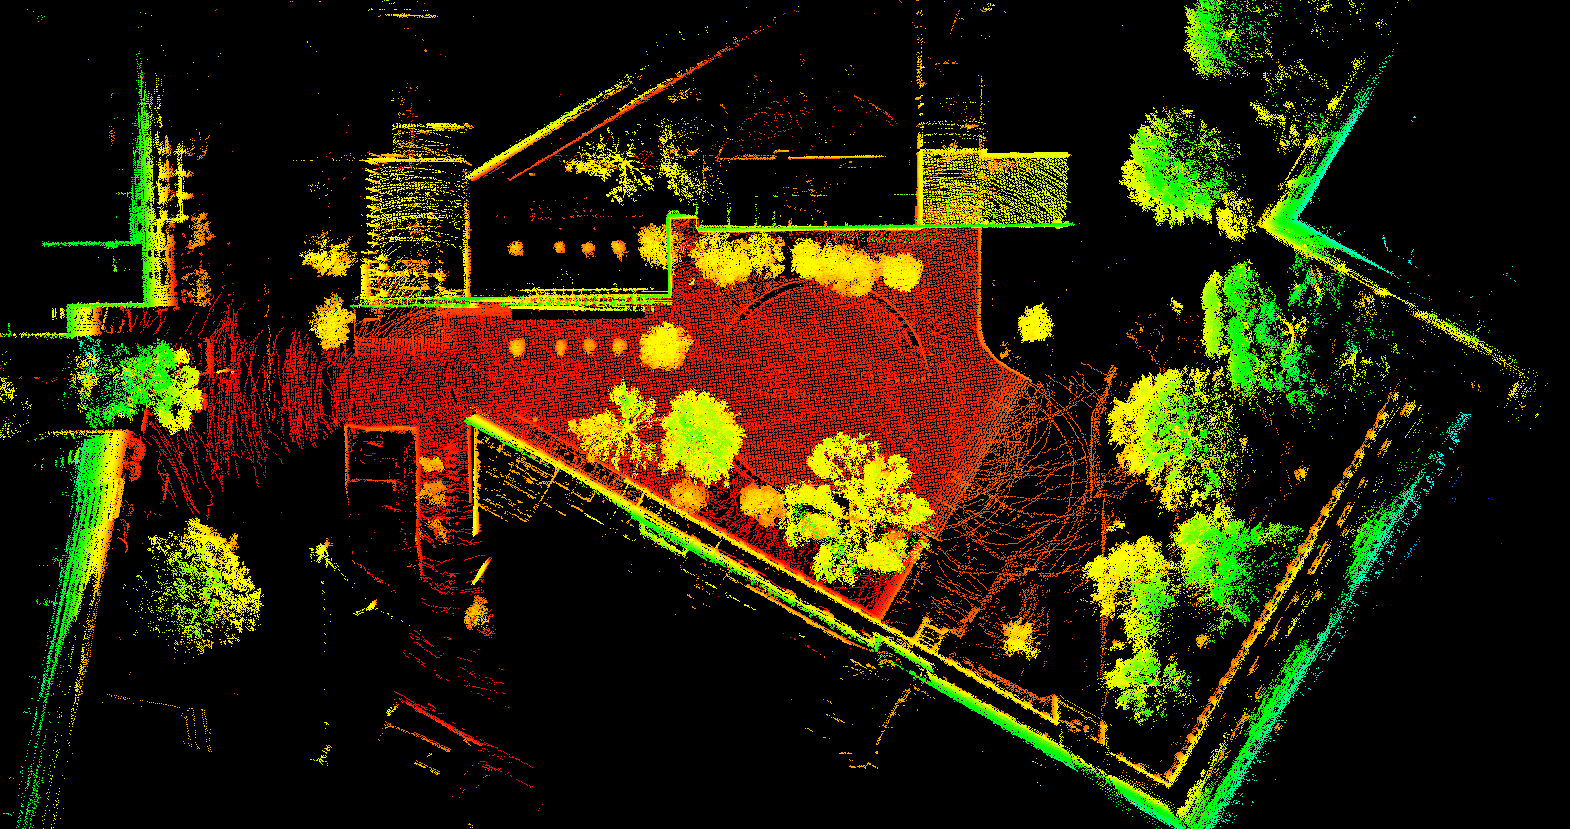
\includegraphics[width=.95\linewidth]{pictures/05/courtyard/ndt/ndt_map_courtyard}}
  \caption{NDT mapping on the courtyard}
  \label{fig:pevndtcou}
\end{figure}

\begin{figure}[h!]
  \centering
  \frame{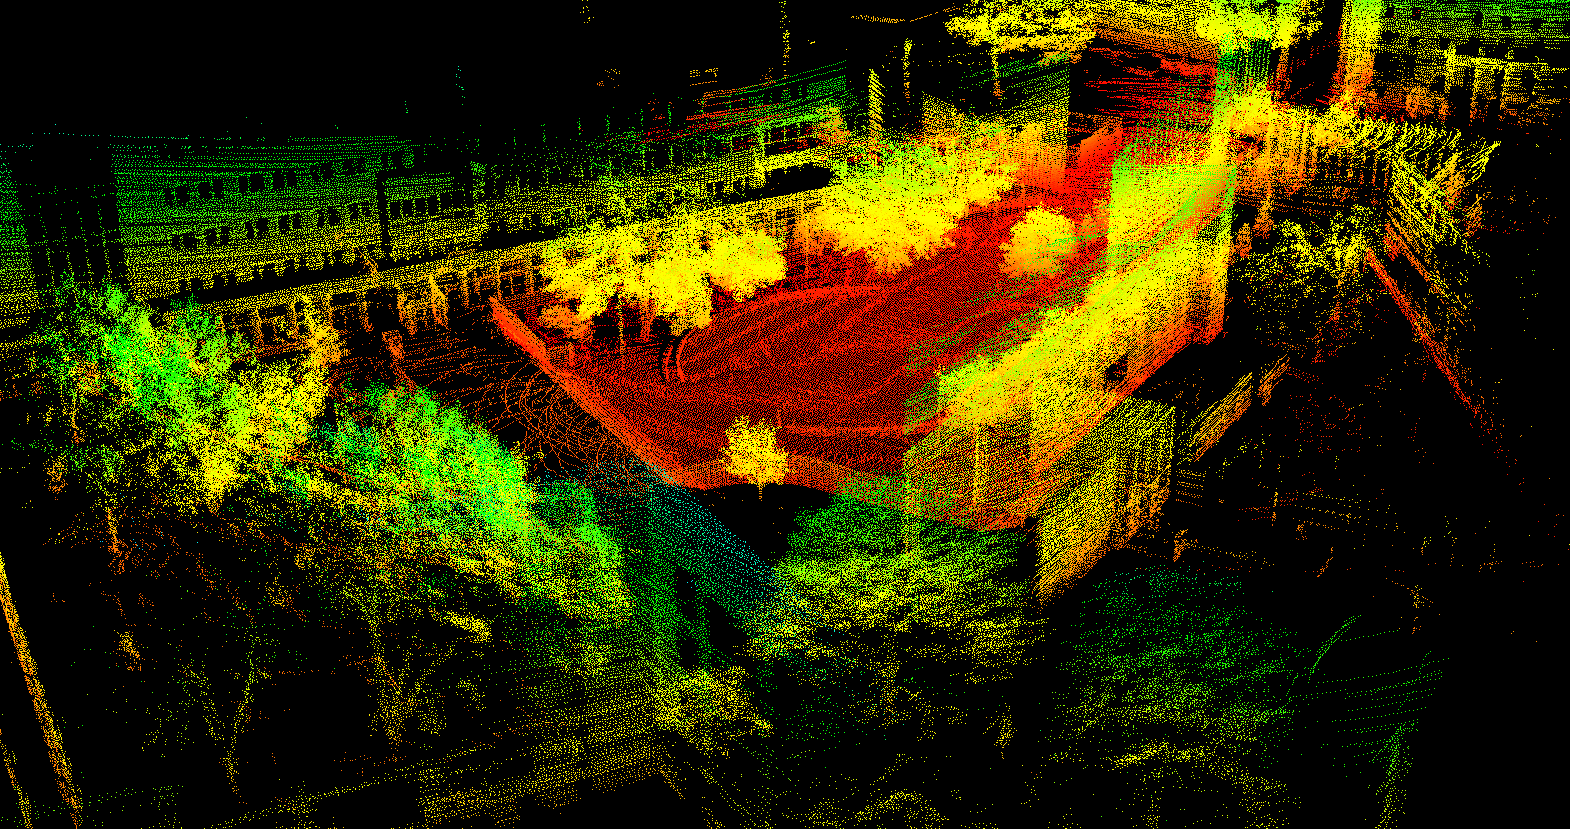
\includegraphics[width=.95\linewidth]{pictures/05/courtyard/ndt/ndt_map_courtyard_detail2}} \\
  \caption{Detail of the result of NDT mapping}
  \label{fig:pevndtcoudet}
\end{figure}

When performing localization with these pointclouds, a voxel grid filter will need to be applied. The tool developed for that purpose can be found on \href{https://github.com/yagoliz/pcd_filter}{Github}.

\subsection{Taipei's Air Force Base (TAF)}
Taipei's Air Force used to have a 1 km\textsuperscript{2} area in the city of Taipei, Taiwan for their military operations, but in the last decaade it was transformed into an innovation space. With the permission of Taipei's government, the PEV was allowed to test on the area shown in \autoref{fig:tafsat}
\begin{figure}[h!]
  \centering
  \frame{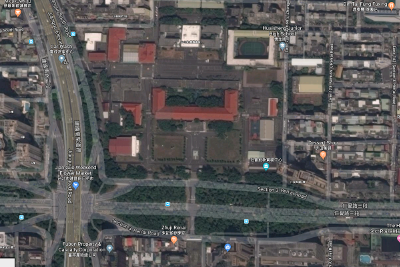
\includegraphics[width=\linewidth]{pictures/05/tafsat}} \\
  \caption{Aerial view of TAF}
  \label{fig:tafsat}
\end{figure}

The specific region recorded is the front part, since it features bike lanes and pedestrian walks, thus making it an interesting area to test how the vehicle adapts to urban real--life scenarios.

\parunder{Hector on TAF} As in previous cases, \autoref{tab:pevhectortaf} summarizes the tested approaches:
\begin{table}[h!]
  \centering
  \begin{tabular}{lc}
    \hline
    \textbf{Parameter} & \textbf{Range} \\ \hline
    Default & - \\ \hline
    Linear update rate & {[}0.1-1.0{]} \\ \hline
    Angular update rate & {[}0.1-1.0{]} \\ \hline
  \end{tabular}
  \caption{Tests with Hector on TAF}
  \label{tab:pevhectortaf}
\end{table}

In \autoref{fig:pevhetafvar}, results of the SLAM are provided. It is notable the quality of the maps obtained in this case compared to the courtyard. This is due to the fact that even though it is a longer path, the PEV is always surrounded by feature--rich environments, thus resulting in low localization errors. \clearpage

\begin{figure}[t!]
  \centering
  \subfloat[Default values]{\frame{\includegraphics[width=\linewidth]{pictures/05/taf/hector/nodomdefault}}} \\  
  \subfloat[Linear update of 0.2 m]{\frame{\includegraphics[width=\linewidth]{pictures/05/taf/hector/nodomlinear02}}} \\
  \subfloat[Angular update of 0.4 rad]{\frame{\includegraphics[width=\linewidth]{pictures/05/taf/hector/nodomangular04}}} \\ 
  \caption{Hector on TAF}
  \label{fig:pevhetafvar}
\end{figure} 

\clearpage
The default map has a small error on the turn of the left part, which is shortened with regards to the actual road, but it is mitigated by increasing the linear and angular update rates.

\parunder{Cartographer on TAF} With regards to Cartographer, the reader might have noticed that it is more sensible to parameter changes than Hector or Gmapping. For TAF, the best combination of parameters achieved on the courtyard was kept and the results are shown in \autoref{fig:pevcartotaf}

\begin{figure}[h!]
  \centering
  \subfloat[Best result with IMU]{\frame{\includegraphics[width=.95\linewidth]{pictures/05/taf/cartographer/cartographerimubest}}} \\  
  \subfloat[Best result without IMU]{\frame{\includegraphics[width=.95\linewidth]{pictures/05/taf/cartographer/cartographernoimubestfaster}}} \\
  \caption{Cartographer on TAF}
  \label{fig:pevcartotaf}
\end{figure} 

Again, the best results are achieved without IMU. And the reason that could explain this is the IMU discalibration, but nothing was seen on the trajectories with or without inertial measurement.

\parunder{NDT on TAF} Lastly, the results for NDT mapping on TAF are shown on \autoref{fig:pevndttaf} and \autoref{fig:pevndttafdet}. Each map took 1 hour to process, taking up 5 GB of the system memory. The resulting pointclouds had a size of $\sim$350 MB so in order to display them, a voxel grid filter had to be applied as mentioned previously.
\begin{figure}[htb]
  \centering
  \frame{\includegraphics[width=\linewidth]{pictures/05/taf/ndt/ndt_map_taf}}
  \caption{NDT mapping on TAF}
  \label{fig:pevndttaf}
\end{figure}

\begin{figure}[h!]
  \centering
  \frame{\includegraphics[width=\linewidth]{pictures/05/taf/ndt/ndt_map_taf_detail3}} \\
  \caption{Detail of the result of NDT mapping}
  \label{fig:pevndttafdet}
\end{figure}
